\documentclass[11pt]{article}

\usepackage{color}
\usepackage{caption}
\usepackage{amsmath}
\usepackage{amsthm}
\usepackage{amsfonts} 
\usepackage{amssymb}
\usepackage{multirow}
\usepackage[pdftex]{graphicx}
\usepackage{epsfig}
\usepackage{latexsym}
\usepackage{enumerate}
\usepackage{tabularx}
\usepackage{booktabs}
\usepackage{fullpage}
\usepackage{algorithm}
\usepackage{centernot}
\usepackage[noend]{algpseudocode}
\usepackage{setspace}
\usepackage{indentfirst}

\newtheorem{thm}{Theorem}
\newtheorem{problem}[thm]{Problem}
\newenvironment{claim}[1]{\par\noindent\textit{Claim:}\space#1}{}

\newcommand{\R}{\mathbb{R} }
\newcommand{\Q}{\mathbb{Q} }
\newcommand{\Z}{\mathbb{Z} }
\newcommand{\N}{\mathbb{N} }
\newcommand{\C}{\mathbb{C} }
\newcommand{\Prob}[1]{ \mathbb{P} \left[ #1 \right] }
\newcommand{\Given}{\middle|}
\newcommand{\overbar}[1]{\mkern 1.5mu\overline{\mkern-1.5mu#1\mkern-1.5mu}\mkern 1.5mu}

\begin{document}

\title{Visualizing Hillary Clinton's Emails}

\author{
  Yihe Chen \\
  \texttt{yc3076}
  \and 
  Palmer Lao \\
  \texttt{pol2105}
  \and
  Daitong Li \\
  \texttt{dl2991}
  \and
  Ziyue Shuai \\
  \texttt{zs2285}
  \and
  Eric Zhang \\ 
  \texttt{ez2232}
}

\date{\today}
\maketitle
\doublespacing


\section{Introduction}
In light of the recent U.S. presidential election race between candidates Donald Trump and Hillary Clinton, there have been large amounts of interest in the controversy involving Hillary's use of personal email accounts on non-government servers during her previous career as Secretary of State. 
After a number of Freedom of Information lawsuits were filed against the Department of State, the Department of State released on August 31, 2015 nearly 7,000 pages of Clinton's heavily redacted communications in PDF form.

Subsequent to this release, the data science competition website Kaggle released a sanitized version of the extracted content of the emails for public use and analysis. 
Our group was interested in analyzing and exploring this data given its connection to current events at the time.

\section{Objectives}
Our main objective with this project was to reduce the immense dimensionality and volume of the data so that the resulting output could be more easily digested by a data analyst or other interested party. We wanted to find patterns in the data that might be of interest, such as communities of receiving or sending parties that shared certain commonalities. 

We tried to discover such patterns through the application of three methods: Social Network Analysis (SNA), TextRank, and Cluster Analysis.

However, rather than simply report on the results of such analysis, we believed that a more effective way to communicate results and allow for the generation of new insights would be to create an interactive visualization that would empower the user to both view our findings and explore the simplified data at will.


\section{Data Source}
Some 7,000 pages of Clinton's emails were released by the State Department in PDF format.
Kaggle then scraped the text from these PDFs and hosted them as CSVs and SQL databases on the Kaggle Kernels platform.
The dataset contains nearly 8,000 emails sent within Clinton's inner circle from December 2010 to September 2012.

\begin{figure}[h]
  \centering
  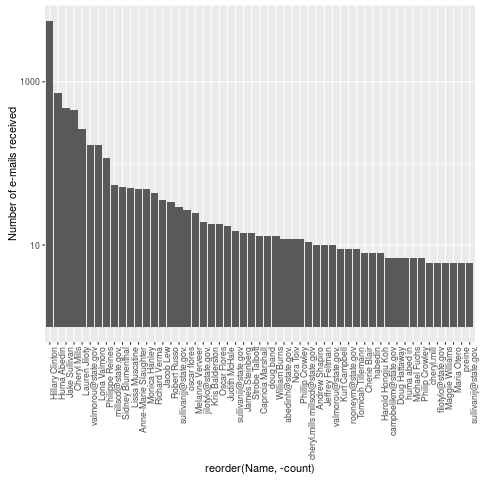
\includegraphics[scale=0.8]{palmer/graphics/num_recvd_histogram}
  \caption{Histogram of how many emails some person has received}
  \label{fig:n_recv_hist}
\end{figure}

\begin{figure}[h]
  \centering
  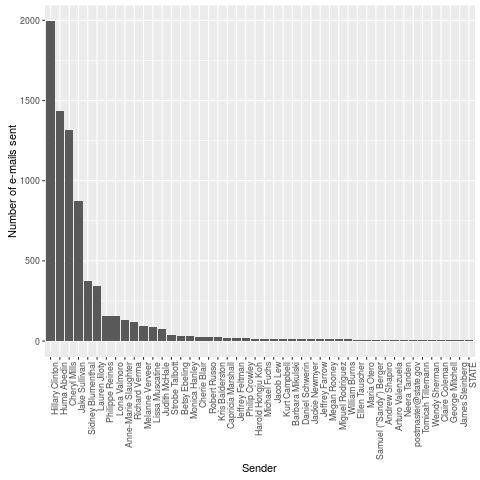
\includegraphics[scale=0.8]{palmer/graphics/num_sent_histogram}
  \caption{Histogram of how many emails some person has sent}
  \label{fig:n_sent_hist}
\end{figure}

Unsurprisingly, the email dataset seems to be Hillary-centric.
In addition, the histogram of emails received seems to be much more highly dispersed than the histogram of emails sent, which may suggest that many emails are sent to multiple people.


Wikipedia summarizes that SNA  is the process of investigating social structures\cite{wiki_sna}. The structure consists of two parts, individuals and interactions, graphically characterized as nodes and edges in the network. So for the purpose of SNA, we reconfigure the original data as two datasets - the Nodes file and the Edeges file (see Figure \ref{fig:node_file} and \ref{fig:edge_file} for snapshots of the data sets).
\begin{figure}[ht]
\caption{Nodes file snapshot}
\label{fig:node_file}
\centering
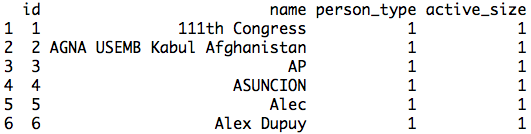
\includegraphics[width=.68\textwidth]{report_node_file}

\caption{Edges file snapshot}
\label{fig:edge_file}
\centering
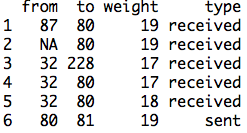
\includegraphics[width=.35\textwidth]{report_edge_file}
\end{figure}

\section{Methodology}

\subsection{An Overview of our Summarization Procedure for one Document}
Because our end goal is to create a visual dashboard for our users, we have to be careful about our bookkeeping while we slice and dice our text data. 
A brief overview of our procedure from end-to-end for one e-mail is as follows:
\begin{enumerate}
\item Split the e-mail into sentences
\item Clean each sentence
\item Represent each sentence as a bag-of-words
\item Run TextRank to get a ranking of the bags-of-words
\item Return the top $k$ sentences from the original e-mail associated with the top $k$ ranking bags-of-words
\end{enumerate}

Of particular importance to our implementation is keeping track of how the bags-of-words are associated with the original sentences from the e-mail, as the bags-of-words are not nearly as informative to the user.

\subsubsection{The TextRank Algorithm}
We treat each e-mail as a self-contained document and attempt to summarize each document using TextRank \cite{textrank}, which is a derivative of PageRank \cite{pagerank} adapted to units of text instead of web pages.

The PageRank algorithm is a way of ranking web pages based on the way that they link to each other.
The algorithm is based on a random walk model of the typical internet user.
We assume the user starts on some arbitrary web page and then either randomly clicks links on the current page or with some re-seeding probability, $d$, navigates to another random web page that was not necessarily linked to from the current one.
The process of such a user's browsing history is clearly Markovian under this assumption.
The addition of the re-seeding probability makes this Markov process irreducible and aperiodic, or equivalently, ergodic \cite{intro-prob-models-ross}. 
Ergodicity allows us to conclude that there exists a so-called stationary distribution over the set of all web pages.
Moreover, this stationary distribution is unique and is the limit of a certain quantity.

The stationary distribution of an ergodic Markov chain has many interpretations.
One is that the distribution assigns probability mass to each state, where this mass is equivalent to the probability that the Markov process is observed in some state after the chain has mixed or lost its dependence on its initial position.
The other is the ``time-average'' interpretation: the average proportion of time-steps a process will spend in some state tends to this state's mass in the stationary distribution.

Web pages that are assigned a large probability mass are thought to be relatively important in the sense that a random web surfer is more likely to visit it.
One can sort the pages by the amount of mass assigned to them by the stationary distribution to get a ranking of pages by this notion of importance.

To turn this idea into something that can summarize text, we need to decide on two things.
The first is the notion of an item to rank, or in our case, a unit of text.
The second is the notion of how all items pairwise indicate each other's importance.

A typical choice of unit of text is either sentences or phrases.
We choose to rank sentences for the sake of simplicity.

For text, we might imagine that a sentence that is highly similar to many of the other sentences is important in the sense that it may mix the contents of the most sentences to provide an insightful summary of the entire document.
Naturally, we might choose to define the transition matrix of the Markov chain over sentences by the similarity between sentences, which now reduces our problem to figuring out a measure of pairwise similarity between sentences.

A naive view of sentences is to think of them as sets or multisets of words.
An easy measure of similarity over sets $S_1$, $S_2$ is the Jaccard similarity:
\begin{equation*}
  J(S_1, S_2) \triangleq \frac{|S_1 \cap S_2|}{|S_1 \cup S_2|}
\end{equation*}
which can easily be extended to multisets \cite{wiki:Multiset}.

We opt to use the recommendation of the original TextRank paper \cite{textrank}:
\begin{equation*}
  \text{Similarity}(S_1, S_2) \triangleq \frac{ | \{ w_k | w_k \in S_1 \& w_k \in S_2 \} |}{\log(|S_1|) + \log(|S_2|)}
\end{equation*}

although there are many other variations that we did not have the chance to evaluate \cite{textrank-sim-var}.

To actually compute the TextRank of a document represented as a collection of bags-of-words, we perform the following procedure:
\begin{enumerate}
\item For each pair of sentences $S_i$ and $S_j$, compute their similarity $\text{Similarity}(S_i, S_j)$ and store it in a matrix as entry $\tilde{M}_{ij}$.
\item Normalize $\tilde{M}$ to get a transition matrix $M$, representing a Markov chain over sentences.
\item Starting with an initial guess of the stationary distribution $R_0$, iteratively compute 
  \[
    R_{t+1} = dMR_t + \frac{1-d}{N} \mathbf{1},
  \]
where $d$ is the re-seeding probability, $N$ is the number of sentences, and $\mathbf{1}$ is a column vector of ones.
\item After enough iterations, $R_t$ will have nearly converged to the true stationary distribution of our damped Markov chain. The rankings of the probabilities in $R_t$ can be regarded as the TextRank of our document.
\end{enumerate}

Running an entirely analogous algorithm on the entirety of the web (a graph consisting of about 322 million edges) took the Sergey Brin and Larry Page, the authors of PageRank, approximately 52 iterations for their ranking to converge, and about 45 iterations on a graph half that size \cite{wiki:PageRank}. 
They concluded that the number of iterations to convergence should be approximately logarithmic in the size of the network.
Since documents tend to create relatively small and dense similarity graphs, we set our number of iterations to a highly conservative 10 iterations.


\subsubsection{Cleaning the e-mails}
Many similarity functions \cite{textrank-sim-var} as well as the one we implemented rely on metrics defined on bag-of-words representations of text.
While the bag-of-words representation is a popular one, it's well known to have many deficiencies that are exacerbated by carelessly processed text.

One consequence of using a bag-of-words is that words that are not a character-for-character match will not be counted as the same.
Much of our text cleaning effort is dedicated to ensuring that words that are indicative of sentence similarity are mapped to the same word, and that words that are not indicative of sentence similarity are removed.

The very first part of cleaning a sentence is simple: we set all of the characters to lowercase, as the capitalization of a word should, in most cases, not change its meaning.

Similarly, we remove any nonalphanumeric symbols from our text, as it seems that the method used to extract the text from the e-mails into a database left many wayward symbols (e.g.\verb!\n!, the newline symbol).
Any nonalphanumeric symbols were turned into spaces and any extraneous whitespace was subsequently deleted.

The next transformation we apply is removing stop words.
Stop words are words that almost every valid sentence in the English language contains, such as ``the'', ``a'', ``as'', or ``for''.
Because stop words are so common, leaving them in the sentences would likely inflate the similarity between many bags-of-words.
Leaving stop words in our text would effectively dilute our measure of how important a sentence is.

Our last problem is that different conjugations of words such as ``run'' and ``running'' will be counted as different although they ostensibly are referring to the same activity.
We can attempt to mitigate this problem by applying a popular text cleaning procedure called stemming \cite{willett2006porter}, which attempts to reduce all words to their roots.
For example, ``running'' would be reduced to ``run'', and ``run'' would stay the same.
This allows us to measure text like ``I am running for president'' and ``a run for office'' as similar despite the fact that (after removing stopwords) none of the words are a character-for-character match.
The \texttt{R} implementation we used is from the \texttt{tm} package, which implements the standard Porter stemming algorithm.


\subsection{Social Network Visualization}\label{sna_nw}
In this subsection, we will present varied ways to visualize the network and some techniques to improve the visualization by using the attributes of the edges and nodes.

\begin{figure}[ht]
\centering
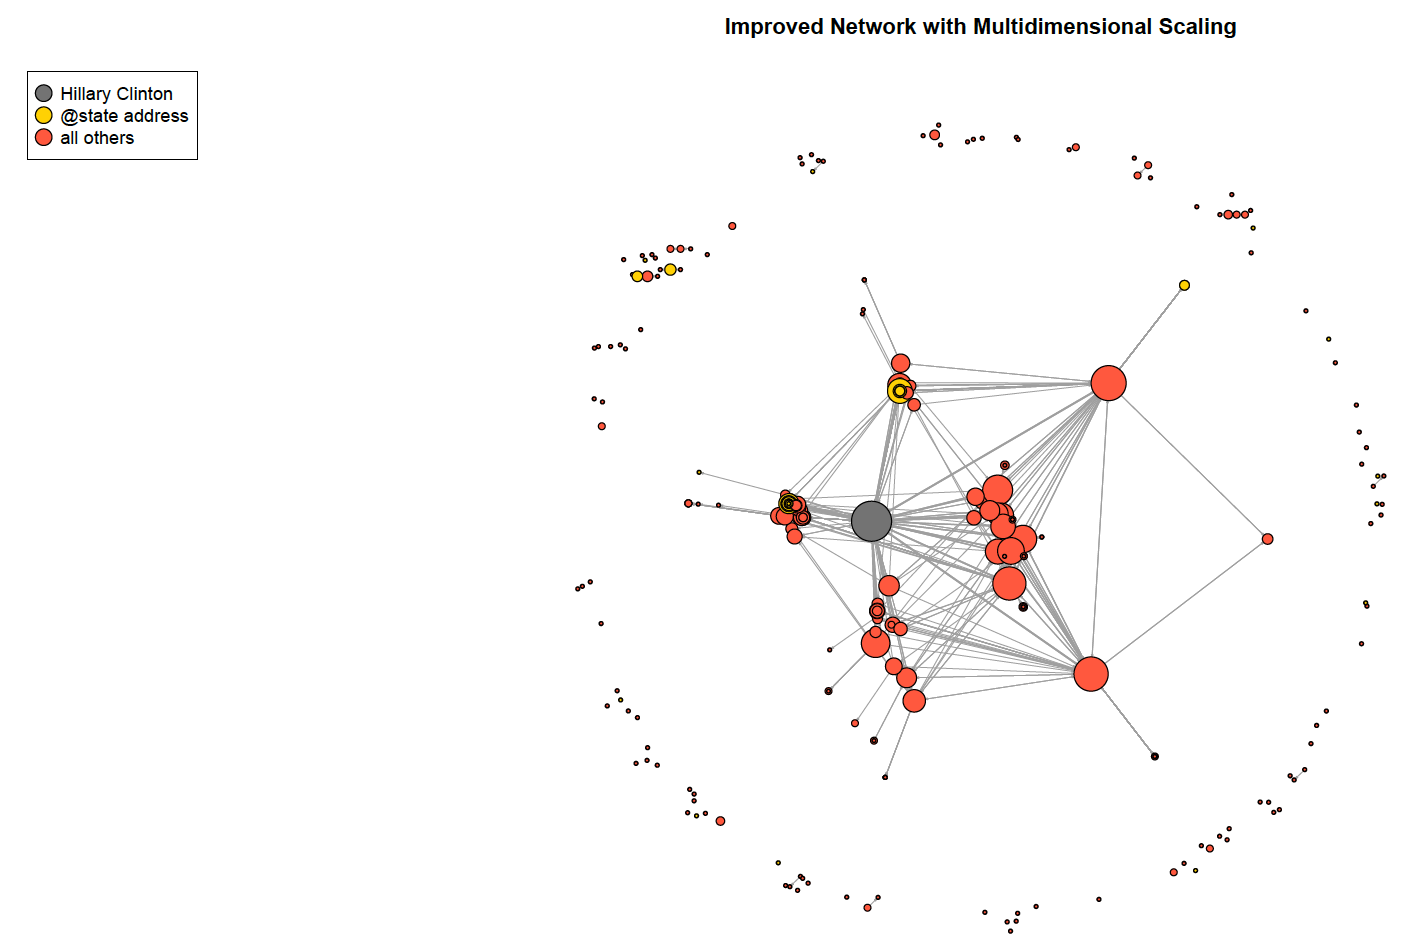
\includegraphics[width = 1\textwidth]{zoe/report_dms_layout}
\label{fig:improvednw}
\caption{Improved Network after Deleting Low-weight Edges}
\end{figure}

One key factor for effective visualization of a network is the graph layout. We have compared $15$ different types of layout and decided to display our network with the Multidimensional Scale layout. The algorithm behind each layout scheme is beyond the scope of our discussion in this report, but we do invite the readers to see Appendix \ref{App:AppendixA} Figure \fbox{empty ref?}  and compare all $15$ layouts we have tested.

The natural choice of color and size for nodes is based on the values of variables ``\verb+person_type+'' and ``\verb+active_size+''. See the legend in Figure \ref{fig:improvednw} to understand the colorcode. Table \ref{tab:node_size} in the previous subsection suggests the distribution of node size is highly skewed, hence we need to rescale it to make it i) more reasonable as iGraph object input as the default is $15$ and ii) have less variance. Inspired by the variance-stablizing transformation, we devised the following rescaling scheme in Equation (\ref{eqt:rescale}). The side-by-side histograms in Figure \ref{fig:rescalenode} demonstrates that this rescaling scheme is effective. The similary log-transform rescaling was also applied to the edge weight, which is also highly skewed.
\begin{equation}
\label{eqt:rescale}
\verb+rescaled active_size+ = \log \verb+active_size+ + 1
\end{equation}

\begin{figure}[ht]
\centering
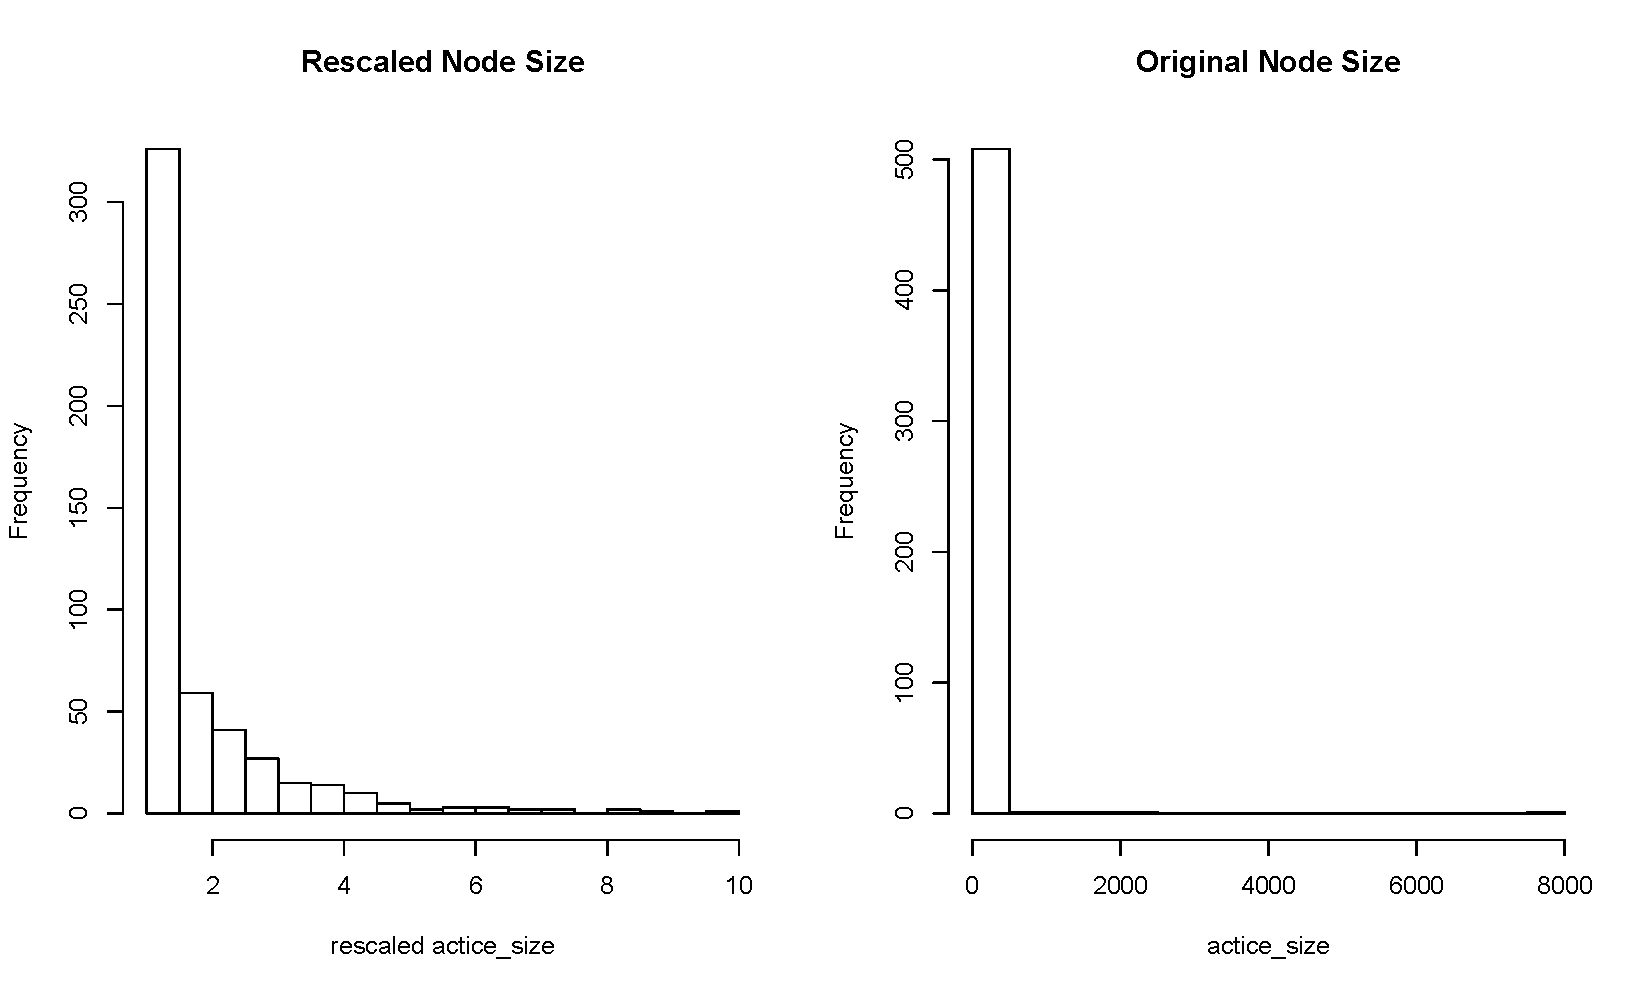
\includegraphics[width=.9\textwidth]{zoe/report_rescaled_size}
\caption{Rescaling of Node Size}
\label{fig:rescalenode}
\end{figure}

\begin{figure}[ht]
\centering
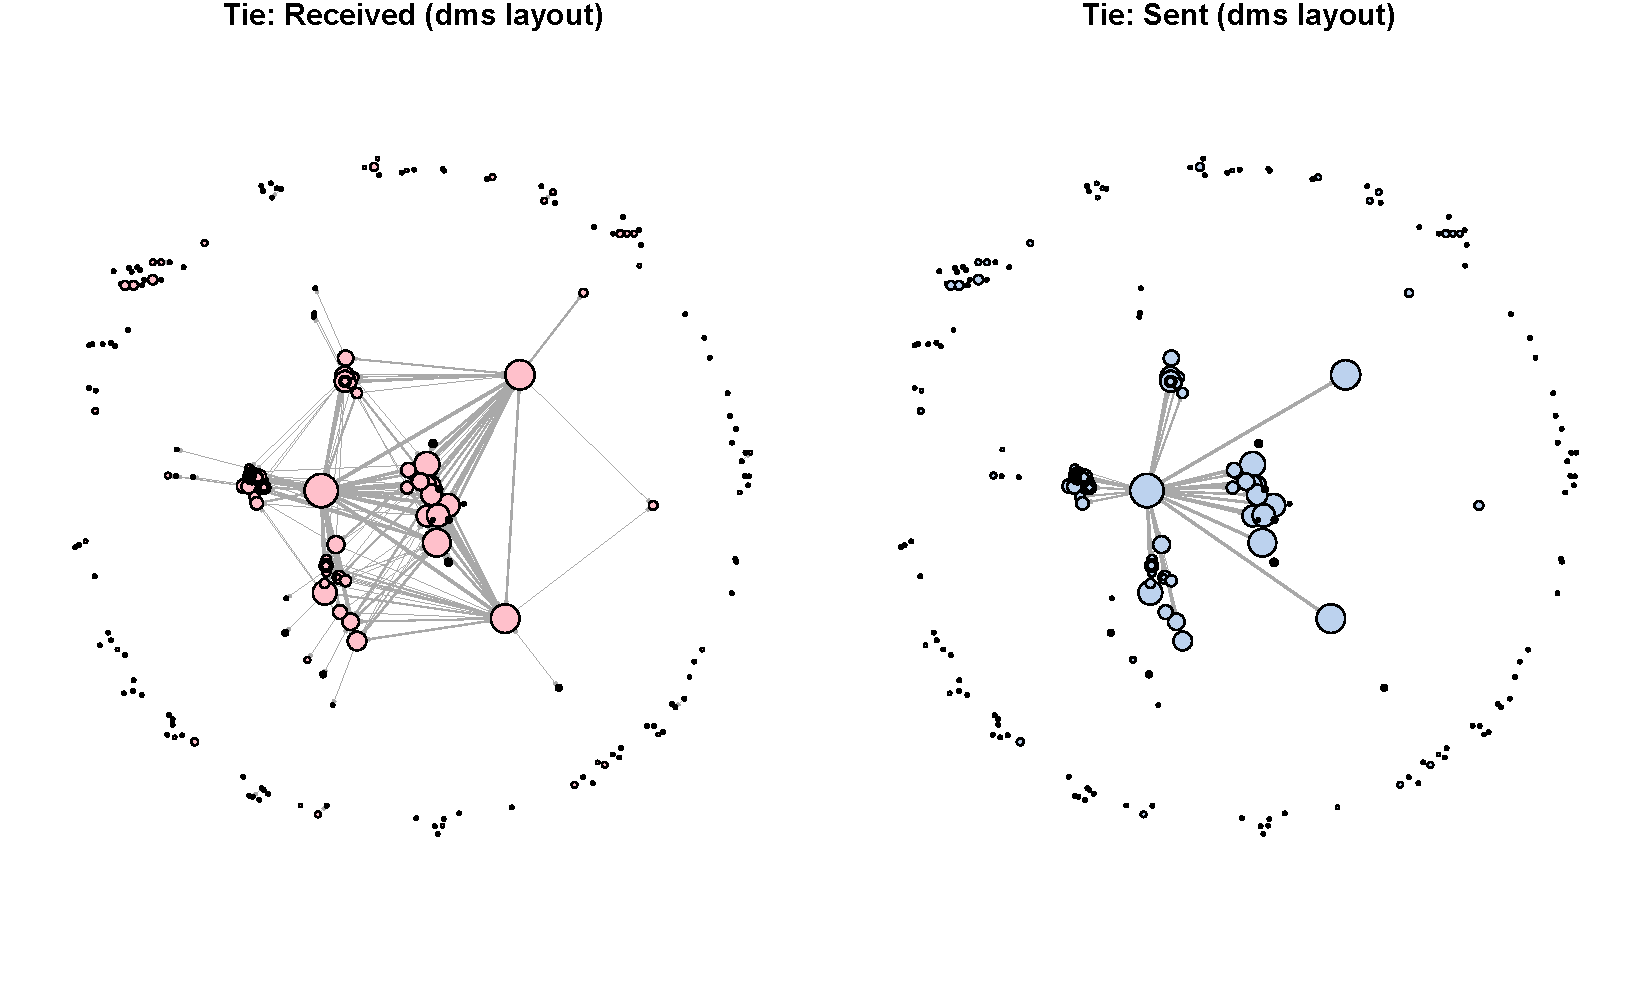
\includegraphics[width=.9\textwidth]{zoe/report_network_compare}
\caption{Visualizing Hillary Clinton Received and Sent E-mails}
\label{fig:splitnw}
\end{figure}

Given a HIllary-centric network, we are also interested in examing the network by the e-mails she received and sent separately. Figure \ref{fig:splitnw} shows the side-by-side sub-network by the node type.

\subsubsection{Network Descriptives and Community Detection}
We examine the Hillary Clinton (abbrev. HC) Email network by studying properties of the smaller units - dyads (pairs) and triads (triangles).   

We first calculate the {\bf density} of this network, which gives us an idea about the extent to which the entire network is connected. The density of a directed network is calculated using Equation \ref{eqt:density}.
\begin{equation}
\label{eqt:density}
\mbox{density }= \frac{\mbox{total number of edges}}{\mbox{number of edges if all nodes were connected}}
\end{equation}
The density of the HC e-mail network is $0.0028<0.01$, which indicates that this network is not at all well connected. That is, less than $10\%$ of the potential pairs within this network have sent or received at least one email from each other. 

A dyad is the smallest possible social group in a network. 
Such a simple unit is worth studying in sociology because two people in a dyad can be linked via some rather exclusive and intimate type of connections, such as ``romantic interest, family relation, ... partners in crime'' \cite{wiki_dyad}.
Among all the $739$ edges in the HC e-mail network, there are $106$ mutual dyads (i.e. double directional links between two individuals), and $527$ asymmetric dyads (the connection only goes one-way). 
Thus, the proportion of mutual dyads is $\frac{2 \times 106}{739}=0.2869$. 
This measure is called {\bf reciprocity}, which in the context of an e-mail network, gives a rough idea about the dynamic of people's interaction as well as information flow through this network. 
That is, among all the connected people, about $30\%$ of the communication were two-way. 

The study of triads is also significant in sociology, as this type of human group is conceptualized to involve more communication interaction than a dyad. According to one source,
``adding an extra person, therefore creating a triad ... can result in different language barriers, personal connection, and an overall impression of the third person.'' \cite{wiki_triad}.
Since the goal of our project is to use SNA as a auxiliary  tool to extract important information (both e-mail content and people's association), the study of triads is beyond the scope of our report. 
However, we do include a brief frequency summary of different forms of triads in our network in the Appendix.

Based on our network, we can use clustering algorithms to find subgroups in the network and thus detect the communities. 
Because we are analyzing a one-person-centered (i.e., HC) network, we expect saliently large weight on this person's node and some of the associated edges, which may cause confounding for community detection. 
Since we are more curious about the unknown in the network, we propose to exclude from the network those edges that originated from HC. Recall that the sub-networks in Figure \ref{fig:splitnw} - the one for received e-mails (Figure \ref{fig:splitnw}, Left) preserves the structure of the whole network (Figure \ref{fig:improvednw}), while there are less edges coming out of the network center.  

We applied the Fast Greedy Modularity Optimization algorithm \cite{greedy_mod} for the details) to the received emails sub-network to find community structure. 
The algorithm yields a lot of single-node communities and one community of extremely large size; this was all expected as we are dealing with a one-individual centered network. 
However, we can examine the communities of size $3$ to $10$ and we do obtain some informative communities that can pass on to the later stage of our project. 
Table \ref{tab:greedy} shows some of the communities we obtain through Modularity Optimization.
\begin{table}
\centering
\begin{tabular}{|l |c| l|}\hline
{\bf ID} & \bf Size & \bf Individuals \\ \hline \hline
\bf 11 & $4$ & \verb+"Bill Clinton"   "Chelsea Clinton"  "Tsakina Elbegdori"    "dad mom"+ \\ \hline
\bf 4 & $6$ & \verb+"Betsy Ebeling"    "Bonnie Klehr"     "Doug Hattaway"    "Robert Russo"+\\
&& \verb+"abdinh@state.gov" "bonnie klehr"+\\ \hline
{\bf 5} & $4$ &\verb+"Kris Balderston" "Mark Penn"       "Marty Torrey"    "Michael Fuchs"+\\ \hline
{\bf 3} & $9$ & \verb+"Harold Hongju Koh"    "Jeffrey Feltman"      "Jennifer Robinson"+\\
&& \verb+"Megan Rooney"         "eichensehr kristen e" "hooke kathleen h"+\\
&& \verb+"johnson clifton m"    "townley stephen g"    "jake.sullivan h"+ \\
\hline 
\end{tabular}
\caption{Communities Detected by Modularity Optimization}
\label{tab:greedy}
\end{table}
From Table \ref{tab:greedy}, we see that with the exception of one individual ``Tsakina Elbegdori'' (the President of Mongolia), people in Community 11 are linked to Hillary Clinton (and each other) via family relation. 
Community 4 involves people who are related to Hillary Clinton's public relations and communications strategy matters. 
For example, Betsy Ebeling is an old and close friend of her who has played an important role in building a positive public image for HC and fighting the perception that Hillary Clinton is untrustworthy. 
Within the same network, we see Bonnie Ward Klehr (with duplicated labels), who not only is a high school friend of Clinton but also designs jewelry for her to wear on the campaign trail. 
We also see other people of similar relation to HC in this community like Doug Hattaway, who was in charge of strategic communications for HC's 2008 presidential campaign, and Robert Russo, who was Director of Correspondences and Briefings for the Hillary for America campaign this year. 

With the communities we detected in our network, we hope to gain a deeper understanding of Hillary Clinton's e-mails from a social interaction perspective and use the output to efficiently browse the large corpus of documents/e-mails and extract as much important information as possible.


\subsubsection{Cluster Analysis}
The social network analysis in the previous section has discovered close relationship between Clinton and a group of her email receivers. The cluster analysis in this section focuses on classifying the receivers' emails in a meaningful way. It is useful to inspect the trends of the language Clinton has used when speaking with different people/groups of people. The clustering analysis is normally useful to categorize large sum of text into groups based on similarities. For exploratory purpose while analysing Clinton's emails, we would like to see if we can categorize based on the language used emails from different circles of people. Due to time limit, we only focuses on the top 10 accounts who have received most emails from Clinton.



\subsubsection{Document-Term Matrix}
To carry out Cluster Analysis, we need to generate a document-term matrix. 
We compiled for each receiver the emails they received together into a document and then cleaned and transformed the text through the following steps:
\begin{enumerate}
\item Convert into lower case. Remove problematic symbols, punctuations and numbers.
\item Remove stop words including 'date', 'can', 'we', 'will' etc. Remove words that are typical in the emails including 'message','sent','original' etc and receivers' names:
\begin{itemize}
\item eg., ``... president nightmare scenarios panetta persuaded renditions tool worth keeping rendition program began carefully monitored form clinton administration bush years transformed ...''
\end{itemize}
\item Convert all documents into a document-term matrix
\begin{itemize} 
\item The matrix has 10 rows representing each email receiver's account; and 20792 columns representing unique words that have appeared in all the email text
\item In each row, if a certain word appears N times the corresponding column would have `N' , `0' if if never appears. The sparsity of the matrix is 74\%, with the count of nonzero entries to zero entries being 53249/155201. 
\end{itemize}
\item Compute Euclidean distance between each pair of documents.
\end{enumerate}
The distance between documents is defined in 20792 dimensional space. To illustrate for instance, suppose we have two documents Doc1 (house, libya, document) and Doc 2 (house, information, release, document). In the document-term matrix, the two documents would be represented by word frequency, eg., we would have Doc1 = (1, 0, 1, 1), Doc2 = (1, 1, 2, 1). The distance between Doc1 and Doc 2 would then be $\sqrt{(1-1)^{2} + (0-1)^{2} + (1-2)^{2} + (1-1)^{2}} = \sqrt{2}$.



\section{Results}
\subsection{TextRank Results}
TextRank proves to be quite useful when summarizing long e-mails.
When prompted for the top 3 sentences of the following text, TextRank picks out the bolded sentences:

\begin{quotation}
`Assume the following two pieces from Dawn in Karachi reached you through other channels, but just to be sure.
The first is exactly the bad story I was worried about.
The second is the Administration's attempt to shoot it down.
\textbf{Bottom line (another four-letter word): ``Whew!''
FIRST STORY
Talks under way for N-deal with US: Haqqani
By Zulciernain Tahir
Monday, 15 Feb, 2010 I 06:02 AM PST I
LAHORE: Pakistan's Ambassador to US Husain Haqqani has said the government has started negotiating with the United
States for an agreement on nuclear technology.}
``The US is not sceptical about our nuclear programme. \textbf{Talks between Pakistan and the US for cooperation on atomic
programmes are under way and we want the US to have an agreement with us like the one it had with India on civil
nuclear technology,'' Mr Haqqani said at a reception hosted by Punjab Governor Salmaan Taseer on Sunday.}
He said Pakistan would get 16 latest F-16 aircraft in June. He said although the expectations of Pakistan and the US with
each other usually did not fulfil, both were indispensable for each other.
``We have to largely depend upon the US for our defence related matters.
India is our main concern as it is buying weapons worth \$100 billion from five countries, including China, and to balance
it our relations with the US are very significant,'' he said and added that India had 5,500 tanks and there was a question
against whom they would be used. ``We cannot be assured by statements that India will not wage a war against us.''
Giving a reason as to why Pakistan had to look towards the US for enhancing its military capacity and capability, Mr
Haqqani said the European countries did not offer soft terms for buying weapons. ``Ties with the US are important for a
secure, stable and prosperous Pakistan.''
Mr Haqqani said Pakistan had also made it clear on the US that it should ensure a strengthened and Islamabad-friendly
regime in Kabul before leaving.
He said Pakistan had sought drone technology from America. ``On one hand our innocent people are losing their lives
while on the other Taliban leaders like Baitullah Mehsud get killed in such attacks,'' he said.
Mr Haqqani said the US wanted to strengthen democracy in Pakistan and aid under the Kerry-Lugar Bill had started
coming from January.
In reply to a question, he said Pakistan's embassy in the US was working on diplomatic and legal aspects in Dr Aafia
Siddiqui case and was making efforts for securing her release or transfer of her case to a Pakistani court.
\textbf{SECOND STORY
No nuclear deal with Pakistan, says US
By Anwar lqbal
Monday, 01 Mar, 2010 I 07:15 AM PST I
WASHINGTON: The Obama administration has told Pakistan it would not get an atomic power plant or a civilian nuclear
deal from the United States.}
A senior US official, while briefing Indian journalists in Washington, said the United States was working closely with
Pakistan to help meet its growing energy needs.
``But nuclear power is not currently part of our discussions,'' and the United States had conveyed its decision to Pakistan,
the official said.
He said the administration had also told Pakistan that ``there is no way they can get a civilian nuclear deal similar to the
one the Obama administration has signed with India.''
The Indo-US civilian nuclear deal, the official said, was ``specific to India only and there is no thinking going on in the
administration to create a template for it.''
\end{quotation}

In our opinion, the three sentences are fairly representative of the entire text.
The entirety of the e-mail is about two stories, and the summary produced captures both headlines as well as another sentence from one of the articles.
\subsection{Cluster Analysis Results}
Looking at the emails dataset, there are 1906 of people who received emails from Hillary. We selected the 10 receivers who received the highest numbers of emails from Clinton directly. We call all email text of one receiver a document. 
A simple word cloud for all 10 documents can be seen in Figure. \ref{fig:wcloud}
\begin{figure}[h!]
    \centering
    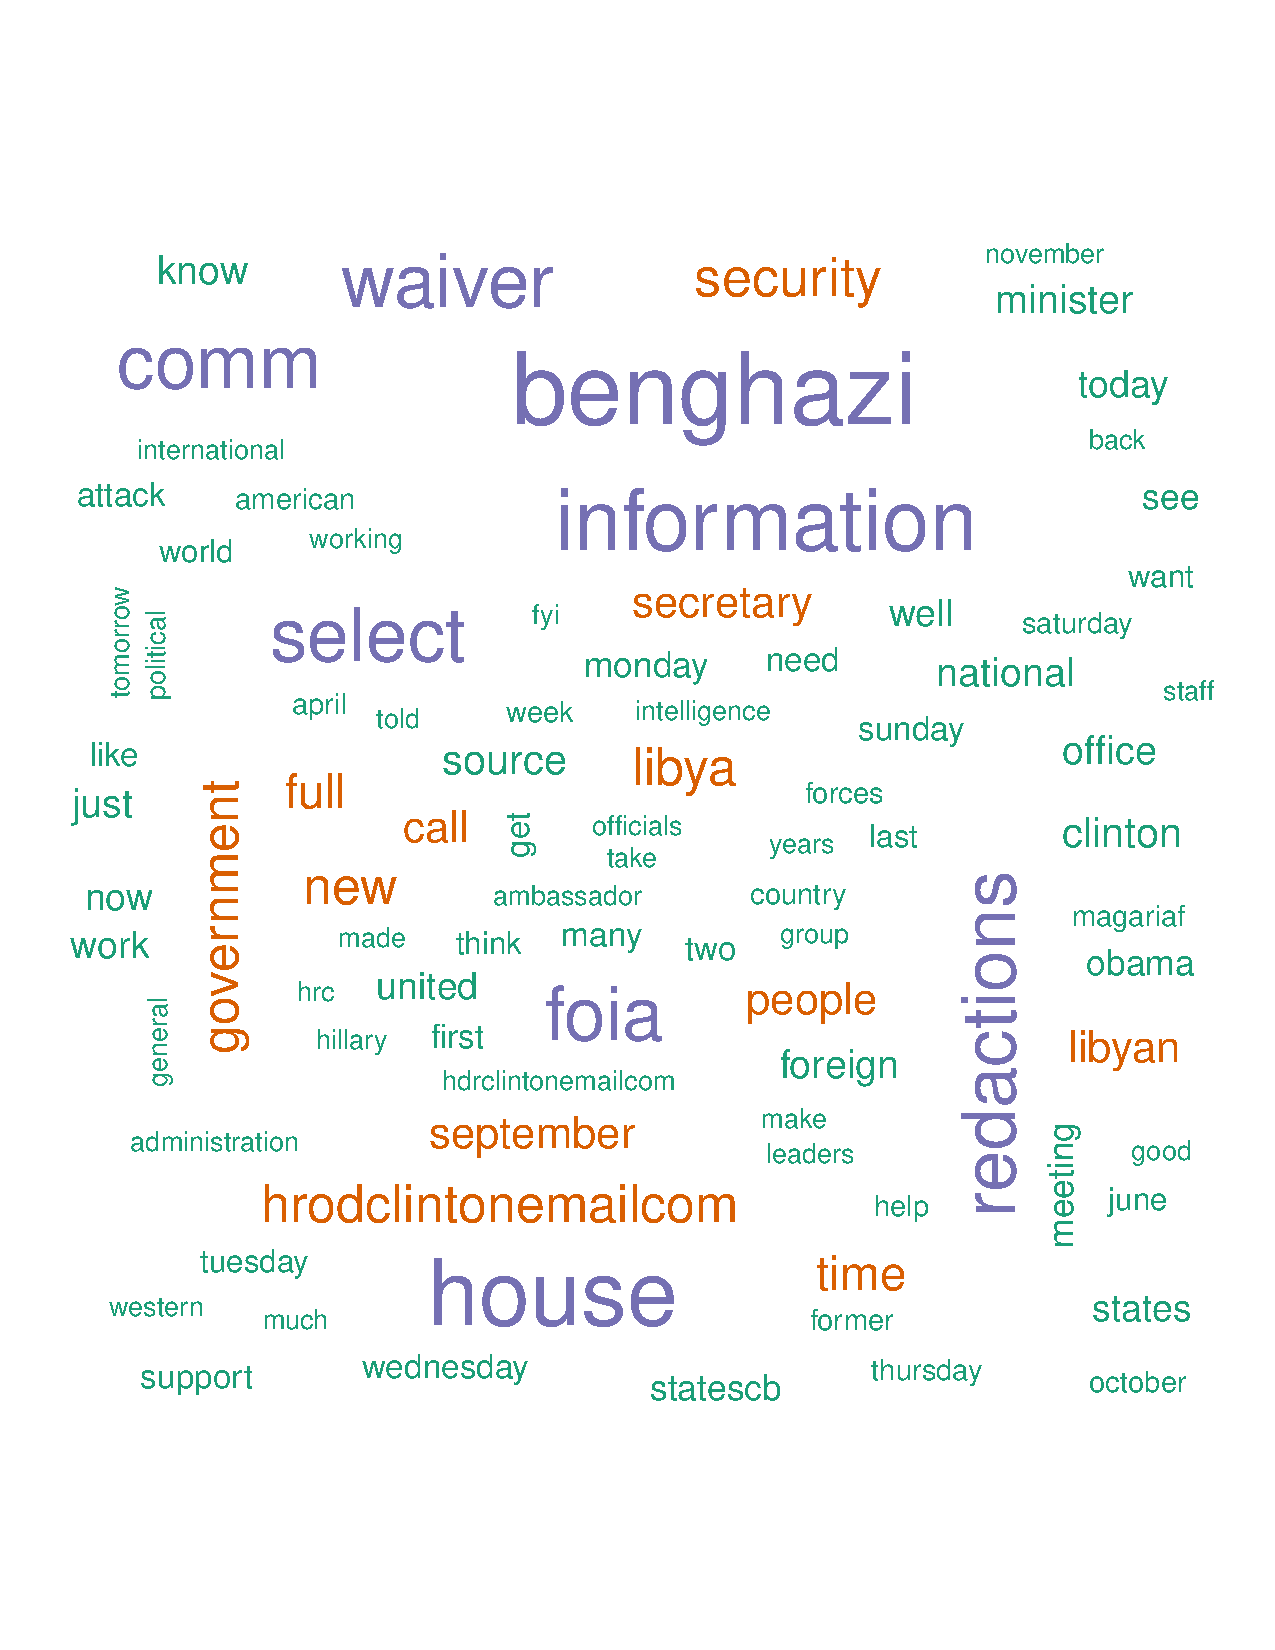
\includegraphics[width=10cm,height=10cm]
    {daitong_and_yihe/wcloud}
    \caption{Word Cloud of Emails}
    \label{fig:wcloud}
\end{figure}

These receivers are a mix of both work email addresses and personal addresses. For example, Huma Mahmood Abedin, the vice chair of Hillary Clinton's 2016 presidential campaign \cite{huma2016}, received 331 emails through her work email address abedinh@state.gov and 31 through her personal email. 
The list of the top 10 email receivers is shown below:
\begin{center}
  \begin{tabular}{ |l| l | c | c |c|}
    \hline
    &Name & Email Type & Frequency & Word count (cleaned)\\ \hline
    1&Huma Mahmood Abedin & Work & 331 & 981 \\ \hline
    2&Cheryl D. Mills & Work & 297 &16145 \\ \hline
    3&Jacob Jeremiah Sullivan & Work & 288 & 1696\\ \hline
    4&Lauren Jiloty & Work & 223 &1993\\ \hline
    5&Lona Valmoro & Work & 129 &8584\\ \hline
    6&Philippe I. Reines & Personal & 49 &15114\\ \hline
    7&Sidney Stone Blumenthal & Personal & 47 &2068\\ \hline
    8&Cheryl D. Mills & Personal & 35 &1786\\ \hline
    9&Monica R. Hanley & Work & 33 &13190\\ \hline
    10&Huma Mahmood Abedin & Personal & 31&6279 \\
    \hline
  \end{tabular}
\end{center}

The typical length of emails varies wildly independent of the number of emails each account received. We can see some patterns from the table above based on the word count. Clinton sent out more lengthy emails to Sidney Blumenthal (personal), Cheryl Mills (personal) and Monica Hanley (work). It makes sense by considering the nature of their connections to HC. 
According to Wikipedia, Blumenthal is a journalist specializing in foreign policy, a former aide to President Bill Clinton, and a long-time confidant to Hillary \cite{sidney2016}. Mills is a lawyer who previously defended Bill Clinton in the 1999 impeachment trial \cite{sidney2016} and Hanley is Hillary's assistant at the state department \cite{zimmermankey2016}.

The table below summarizes the roles or occupations of these 8 key persons in relation to Hillary:

\begin{center}
  \begin{tabular}[h]{|l|l|} 
    \hline
    Roles & Names  \\
    \hline
    \multirow{3}{*}{Special Assistant} 
          & Lauren Jiloty \\ 
          & Lona Valmoro \\ 
          & Monica Hanley  \\ 
    \hline
    \multirow{2}{*}{Senior Policy Advisor} 
          & Philippe Reines \\
          & Jacob Sullivan \\ 
    \hline
    \multirow{1}{*}{Political Journalist} 
          & Sidney Blumenthal \\ 
    \hline
    \multirow{1}{*}{Lawyer} 
          & Cheryl Mills \\
    \hline
    \multirow{1}{*}{Political Staffer} 
          & Huma Abedin \\ 
    \hline
  \end{tabular}
\end{center}

Huma Abedin received the highest amount of emails from Hillary, though these were mainly brief. She served as the Vice Chair for Hillary's 2016 presidential campaign, and was previously the Deputy Chief of Staff to Secretary of State Hillary Clinton from 2009 to 2013 \cite{huma2016}. The two senior advisors also have deep connections to Hillary. Jacob Sullivan specializes in foreign policy and was an advisor to Hillary during the campaign \cite{jake2016}. Philippe Reines served as the Deputy Assistant Secretary of State for Strategic Communications in 2010 and was a senior advisor to Secretary of State Hillary Clinton in 2009 \cite{philippe2016}. Other accounts that have received frequent emails from Clinton are Anne-Marie Slaughter, Richard Verma, Robert Russo, and Lissa Muscatine (speech writer), all of whom received under 30 emails each. 

Although the word counts already reflect Hillary's language style to different people in some sense, we would like to carry out the cluster analysis in terms of text similarities to answer questions like: 
\begin{enumerate}
\singlespacing
  \item Does Hillary talk about similar key issues to certain (group of) people?
  \item Can we separate emails sent to private accounts from the emails sent to work accounts based only on the language used?
\end{enumerate}
\doublespacing
After obtaining the matrix containing the distances between each pair of document, we tried two clustering methods: hierarchical clustering and K-means. 

For hierarchical clustering, we used ward.D or the Ward's minimum variance method. Figure \ref{fig:dendr} is a cluster dendrogram of the top 10 email accounts. The different colors represent the grouping. The height represents the distance between each document. For example, at the distance of 800 we can separate the group into pink and non-pink subgroups. The calculation of distance is explained in the Section 4.2.3.
\begin{figure}[h!]
    \centering
    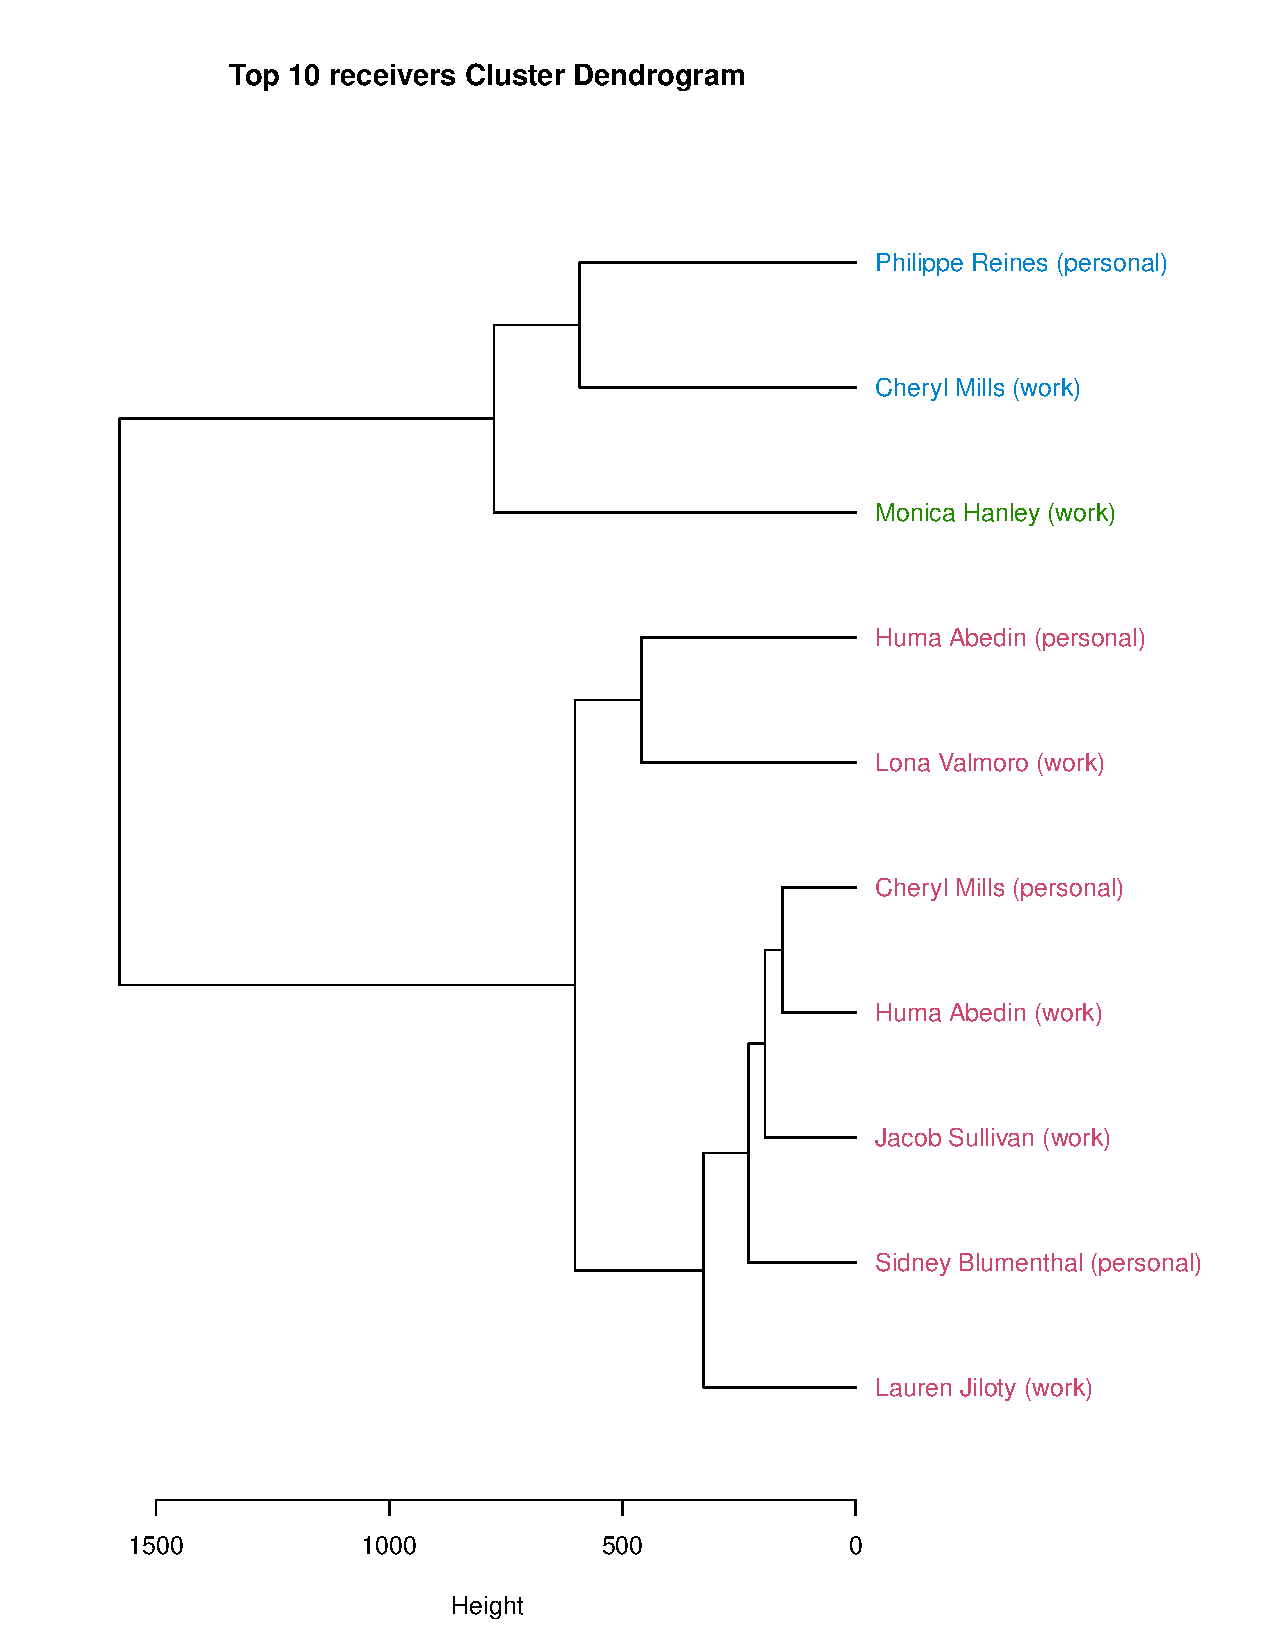
\includegraphics[width=10cm,height=10cm]
    {daitong_and_yihe/clusterp.pdf}
    \caption{Dendrogram of top 10 receiver accounts}
    \label{fig:dendr}
\end{figure}

We can also use K-means to determine the clusters. By plotting the Within Group Variation versus K, we can see from Figure \ref{fig:determine} (in Section 9.3) that K=2 or K=3 might be appropriate group numbers for this dataset.

The cluster plots with K=2 and K=3 can be shown in Figures \ref{fig:c2} and \ref{fig:c3} below. The x and y axes are represented by the first and second components from a PCA analysis. As we can see, the first two components explain more than 95\% of the variance, allowing the clusters to be well separated. 

The results of K-means agree with the results from hierarchical clustering. With K=2, we have Sidney Blumenthal (personal), Cheryl Mills (personal) and Monica Hanley (work) in one group (call it Cluster 1) and the other accounts in the second group. With K=3, we have Sidney Blumenthal (personal), Cheryl Mills (personal) in group one, Monica Hanley (work) in group two, and the other accounts in group three.

\begin{figure}[h!]
    \centering
    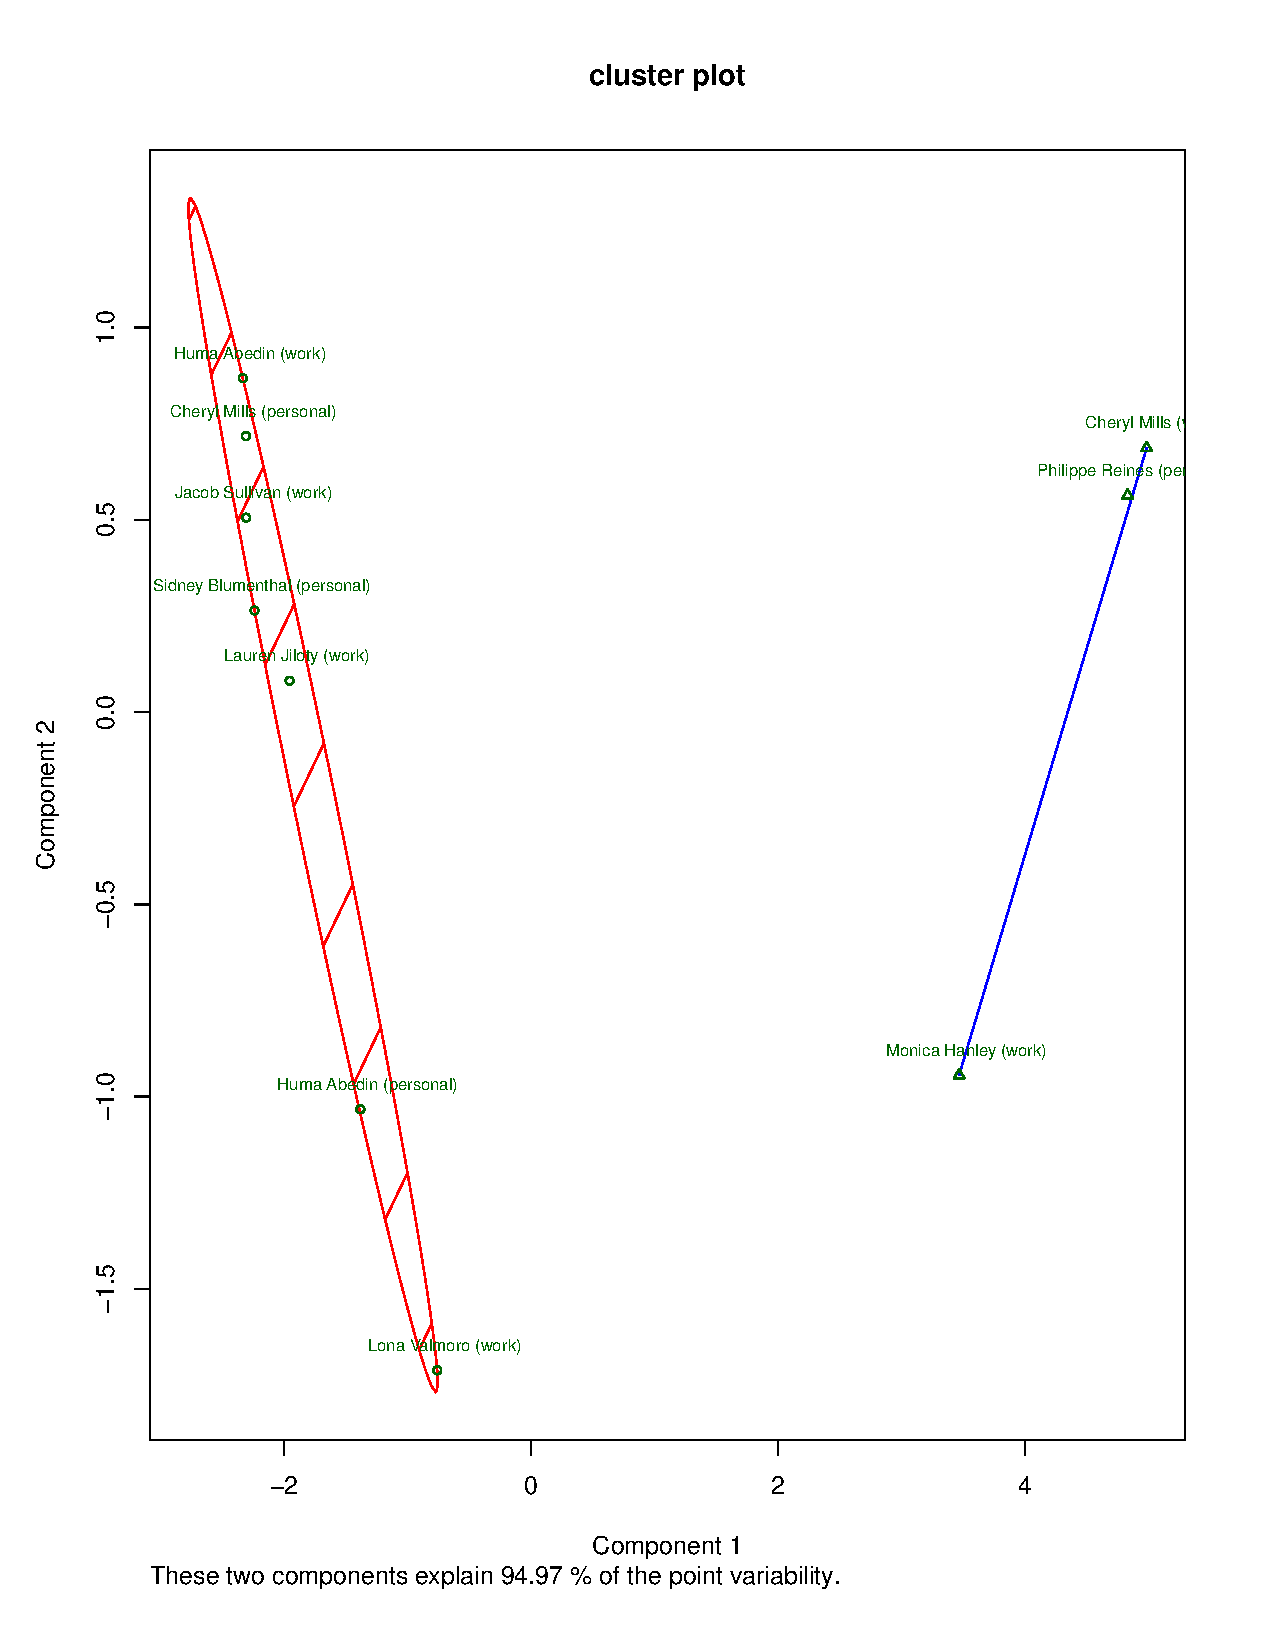
\includegraphics[width=10cm,height=9cm]
    {daitong_and_yihe/c2.pdf}
    \caption{Cluster Plot with K=2}
    \label{fig:c2}
\end{figure}

\begin{figure}[h!]
    \centering
    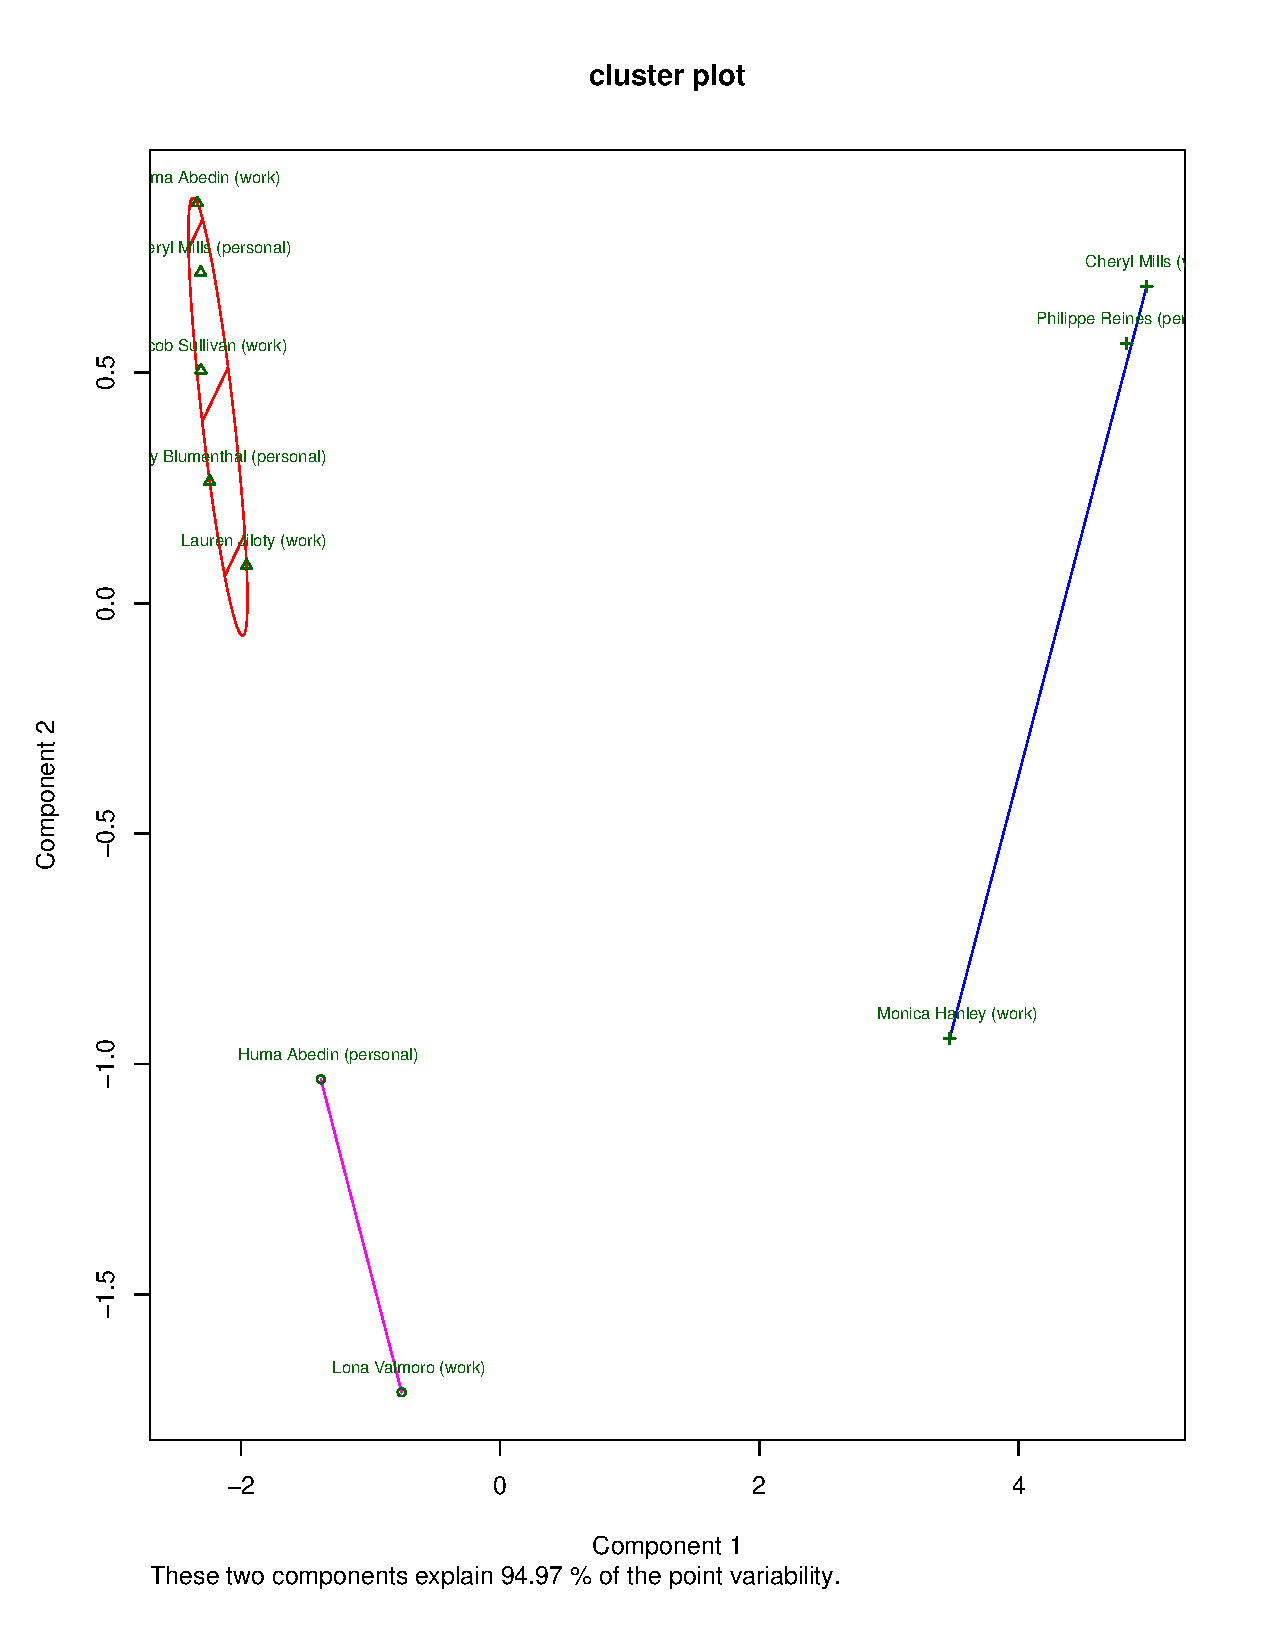
\includegraphics[width=10cm,height=9cm]
    {daitong_and_yihe/c3.pdf}
    \caption{Cluster Plot with K=3}
    \label{fig:c3}
\end{figure}

\newpage
Furthermore, we can inspect the most frequent words mentioned by Clinton to each cluster of receivers. Below are the top 5 words related to each of the two clusters. Both clusters share common words like Benghazi, sensitive and house, although Hillary used the term `agreement' more often with the journalist and the lawyer and the term `release' more frequently with her aides and advisors. 

\begin{center}
\begin{tabular}{ |p{3cm}|p{3cm}|| p{3cm}|p{3cm}|  }
 \hline
 \multicolumn{4}{|c|}{Top 5 Most Frequent Words} \\
 \hline
 Words (Cluster 1)  & Percentage of Occurrence & Words (Cluster 2) & Percentage of Occurrence\\
 \hline
 benghazi & 0.76\% & release  & 0.701\% \\
 house &  0.68\% & benghazi & 0.56\% \\
 sensitive & 0.65\% & house & 0.53\%\\
 information & 0.63\% & information & 0.47\%\\
 agreement & 0.57\% &  sensitive  & 0.46\% \\
 \hline
\end{tabular}
\end{center}



\subsection{Visualization Results}
The social network and summarized text data is combined into a visualization that can be displayed in RShiny. The RShiny dashboard uses the packages visNetwork and igraph. visNetwork is an R package for visualizing networks that allows users to create dynamic and interactive visualizations. Users can physically manipulate edges and nodes in a network graph, select and view nodes by group, and customize the appearance of the network with colors and images. igraph is a set of fast and easy to use network analysis tools in R that allows the user to quickly set up and define network graph relationships that can then be ported over to visNetwork for visualization.

The visualizations were produced by combining the clustering results with the TextRank algorithm.
The clustering results output the set of nodes and their groupings. Then, the TextRank algorithm was applied to the communications between each set of nodes, reducing the large volumes of text for each pair of nodes to a single sentence that would in theory summarize their conversations. The Social Network Analysis results were similarly combined with the TextRank algorithm.

The code for producing these visualizations is included in the Appendices. Below are shown some screenshots of the visualizations when run in RStudio.

\begin{figure}[h]
	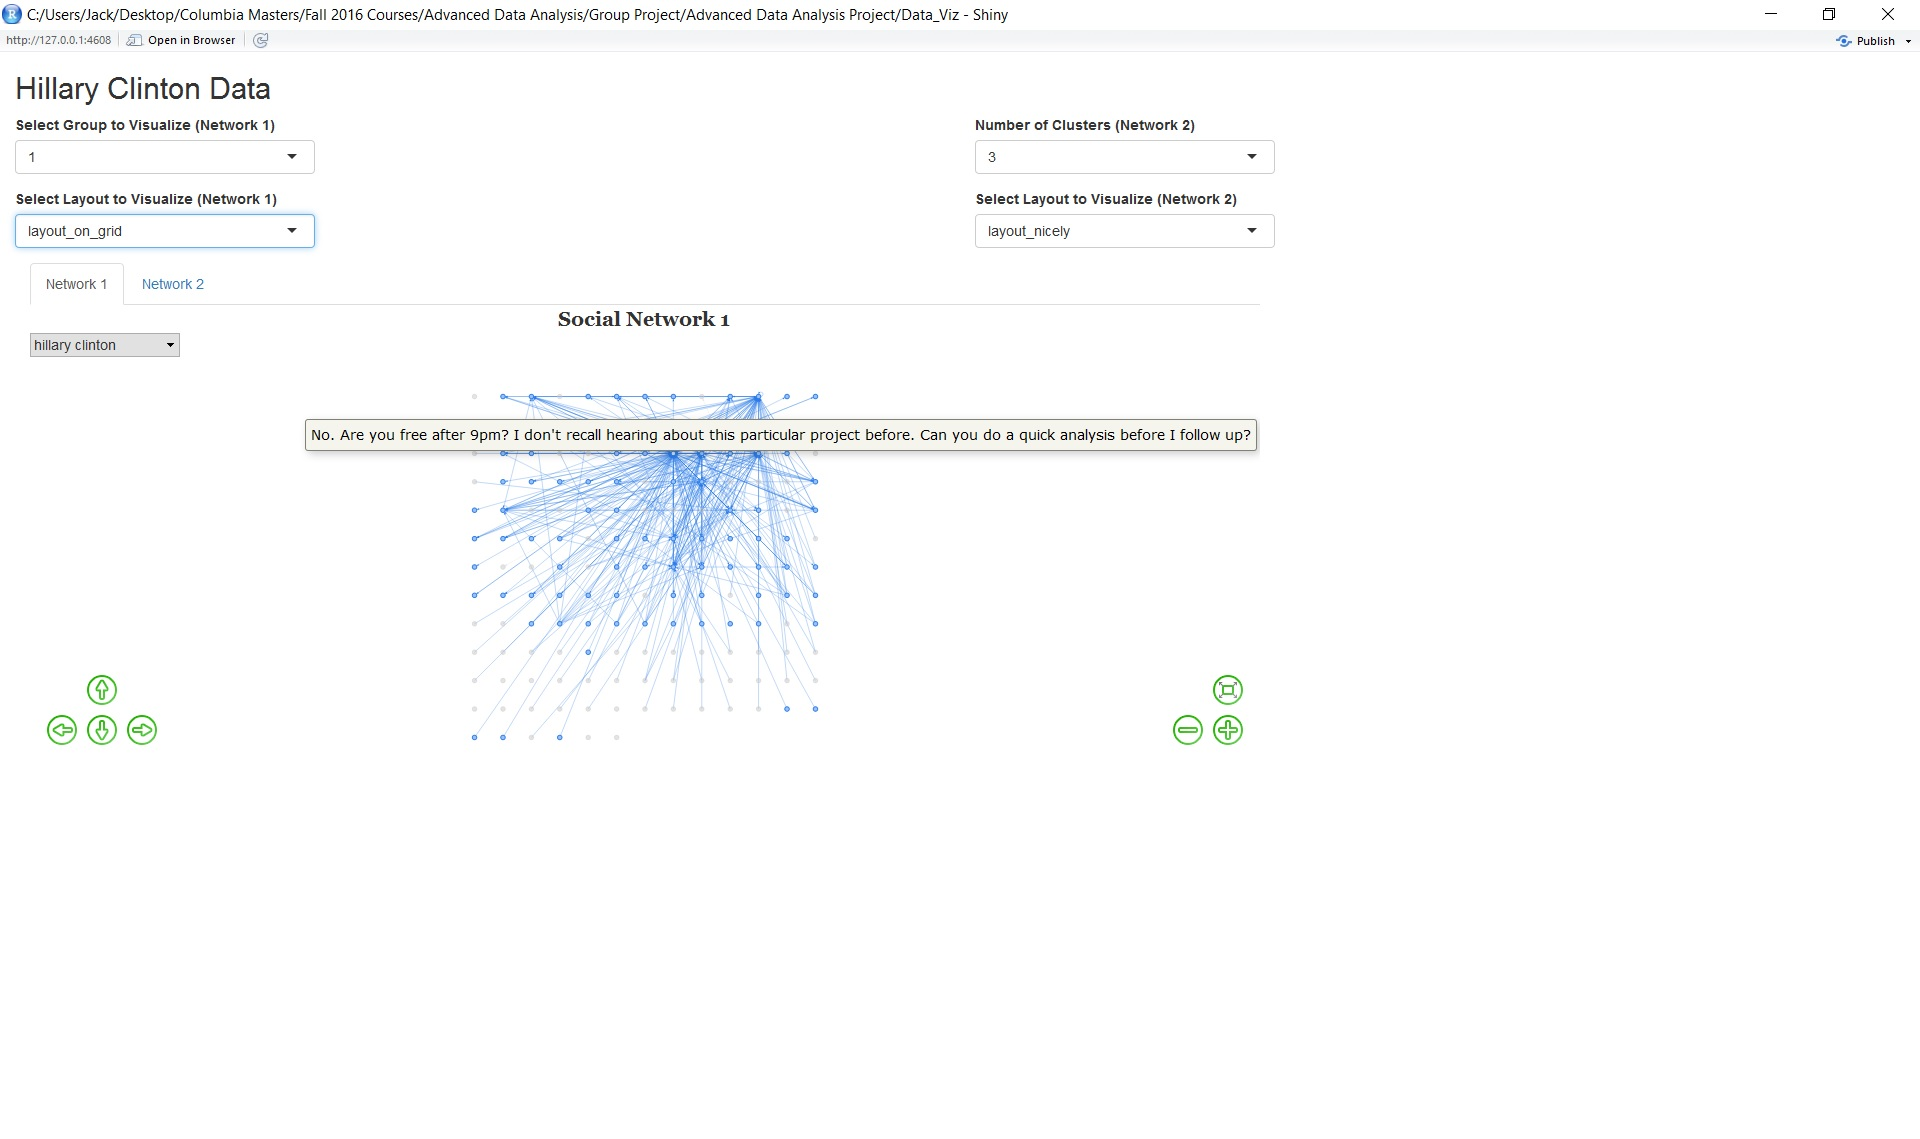
\includegraphics[width=\textwidth]{eric/Viz_Screenshot_1}
	\caption{Hovering the mouse an edges or node in the visualization will cause a tool-tip to pop up that shows the associated summary sentence as determined by TextRank. This figure shows the results of Social Network Analysis combined with TextRank.}
	\label{Viz1}
\end{figure}

\begin{figure}[h]
	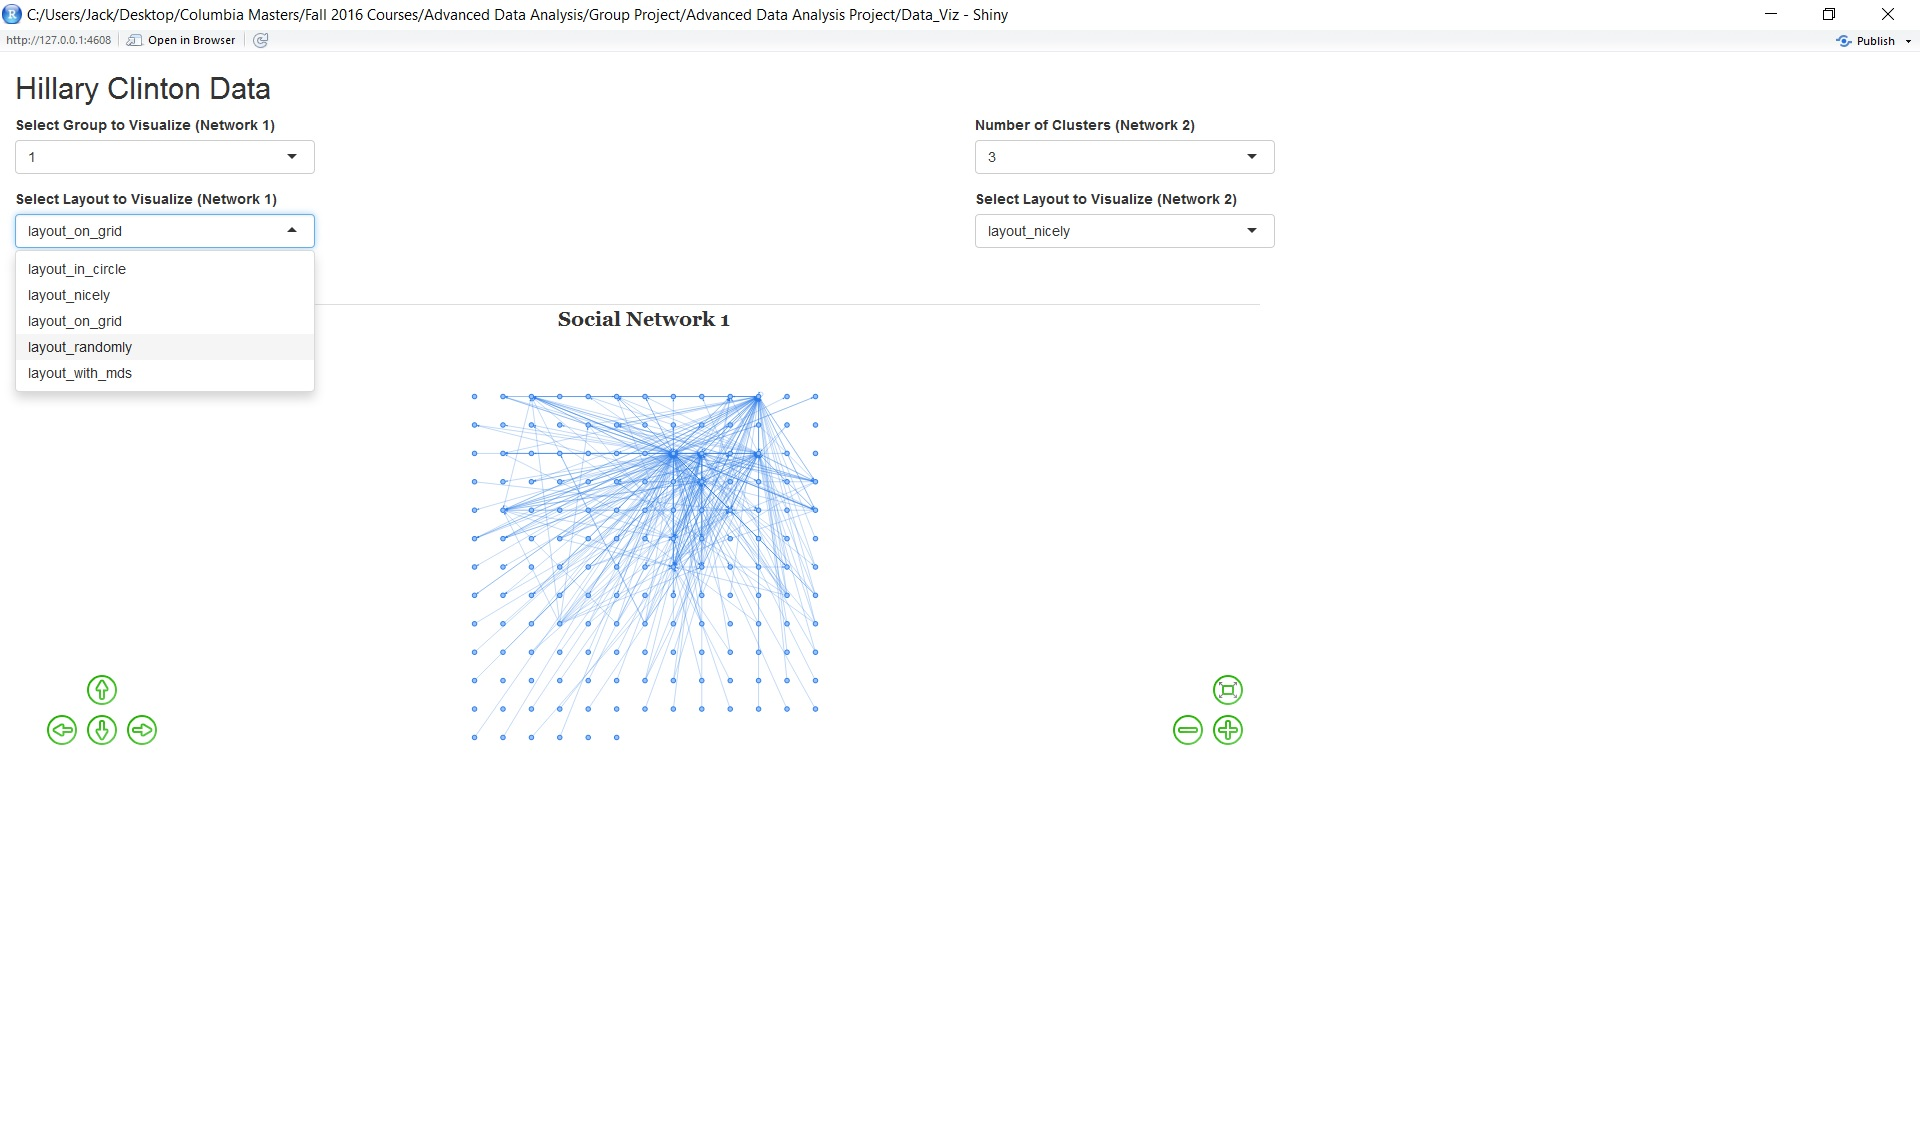
\includegraphics[width=\textwidth]{eric/Viz_Screenshot_2}
	\caption{Showing the various graph layouts available in the visualization}
	\label{Viz2}
\end{figure}

\begin{figure}[h]
	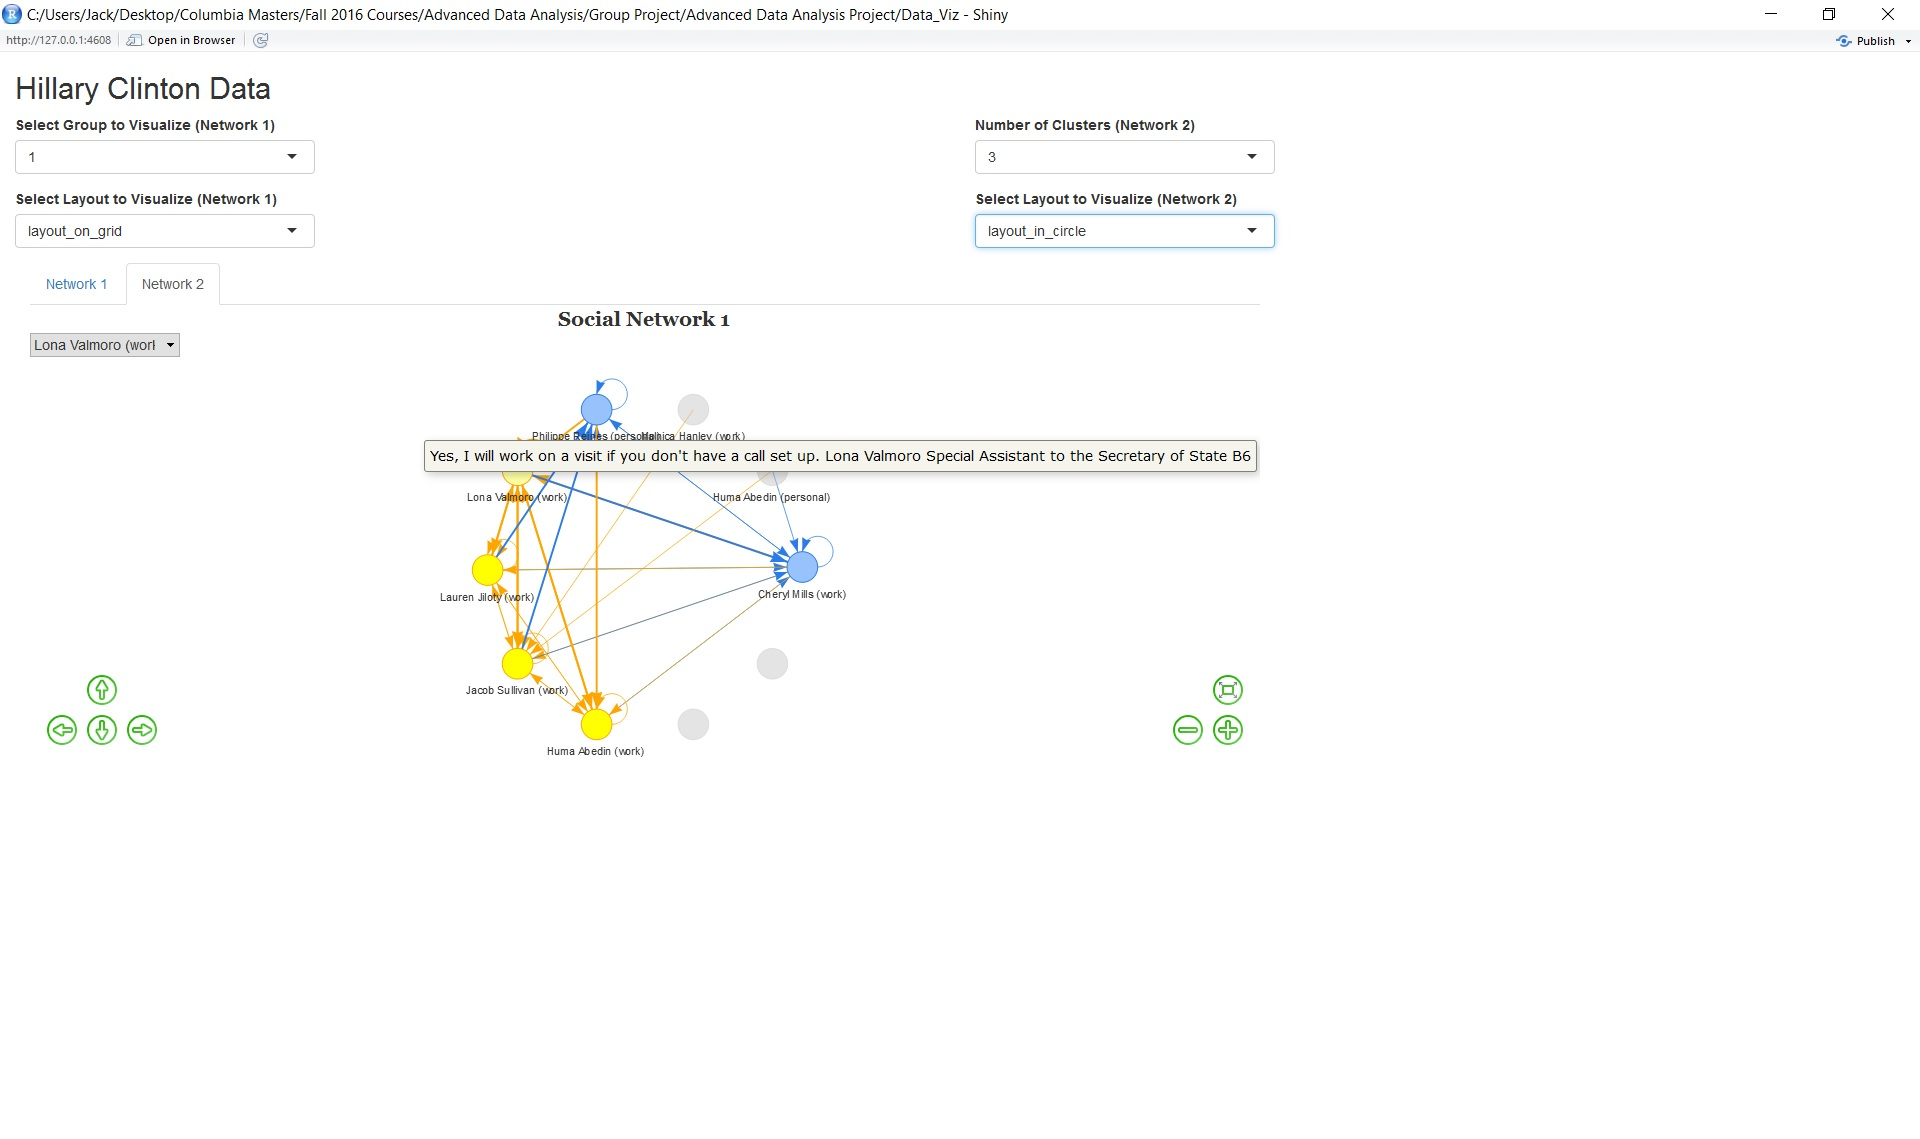
\includegraphics[width=\textwidth]{eric/Viz_Screenshot_3}
	\caption{This figure shows the results of Clustering Analysis combined with TextRank.}
	\label{Viz3}
\end{figure}

\begin{figure}[h]
	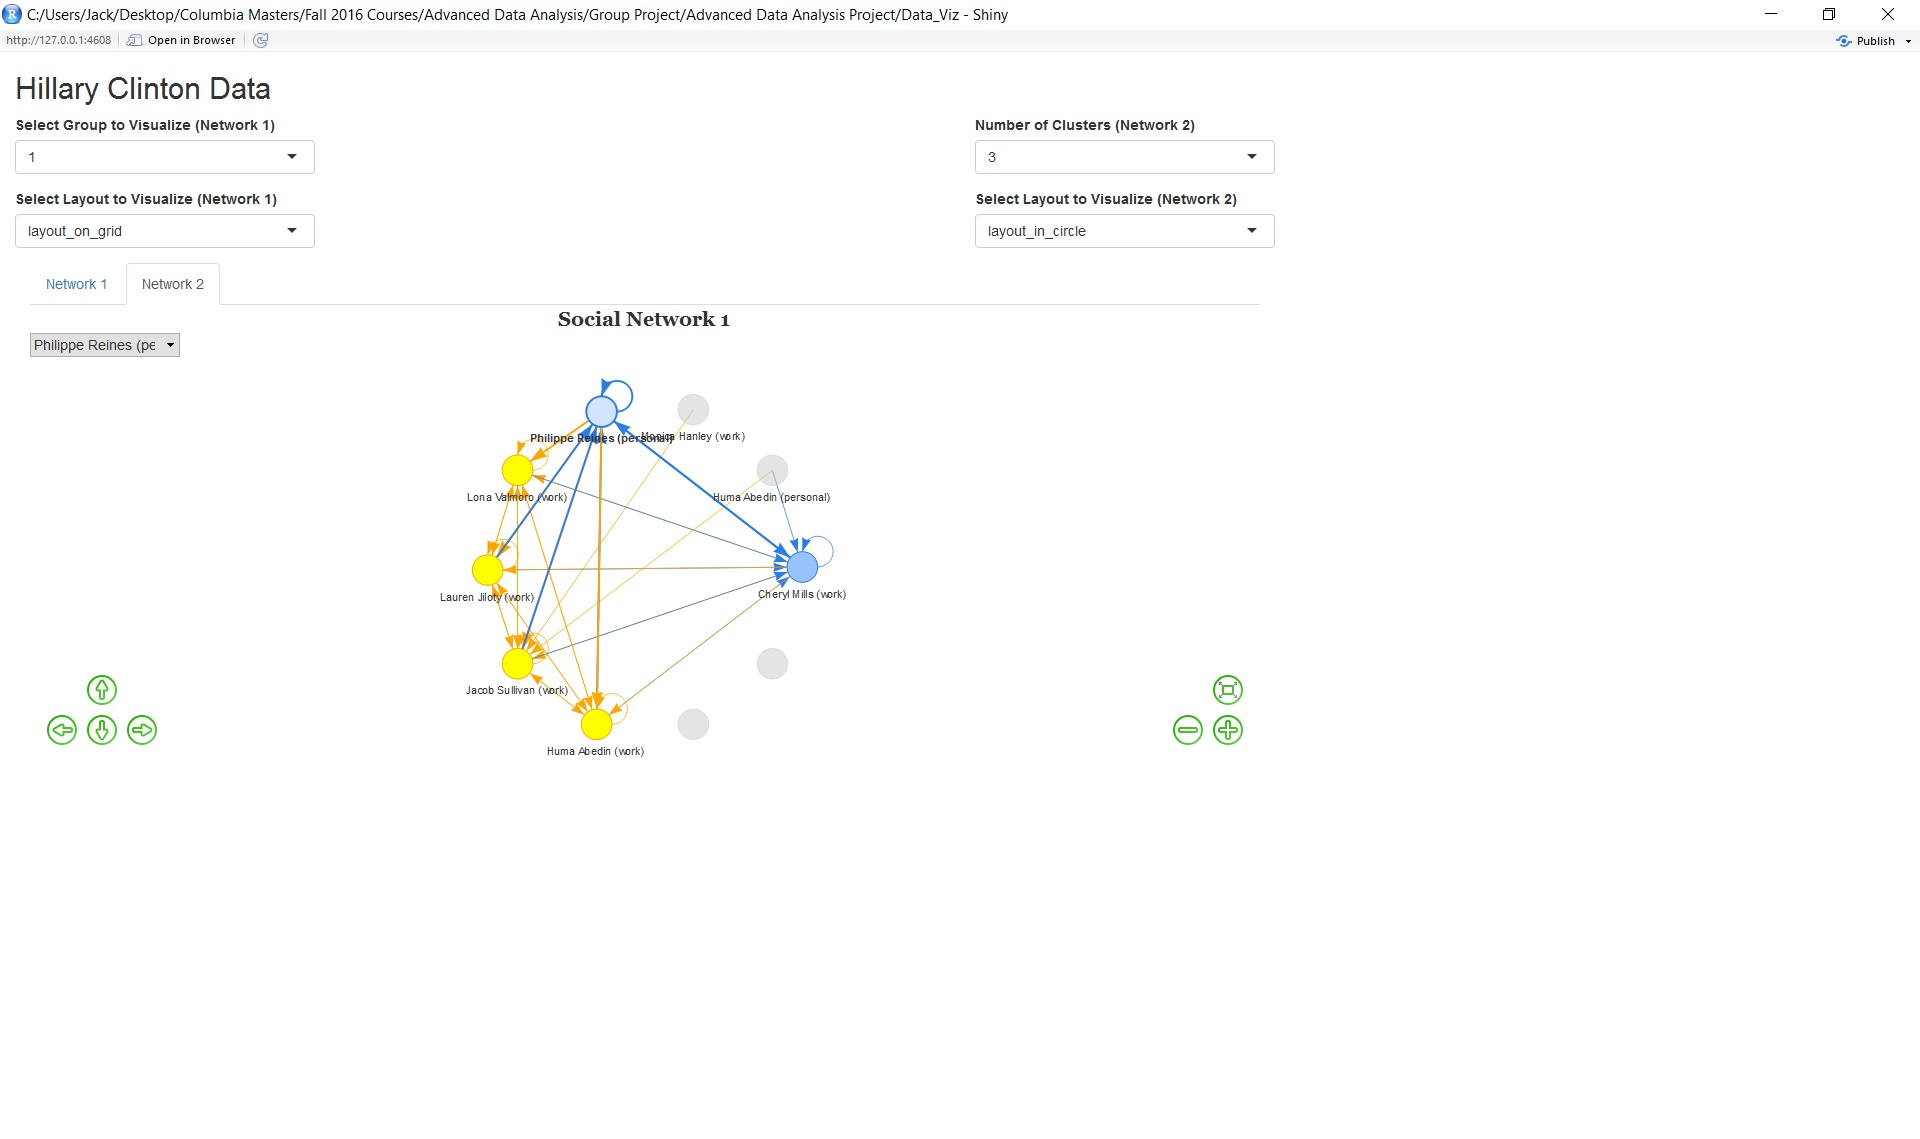
\includegraphics[width=\textwidth]{eric/Viz_Screenshot_4}
	\caption{The visualization allows the user to interact with an manipulate graph nodes. The figure above shows what this looks like.}
	\label{Viz4}
\end{figure}


\section{Model Validation}
\subsection{Choice of Hyperparameters for TextRank}
There are a few parameters to choose for TextRank.
For any use of TextRank at all, one must certainly decide on the re-seeding probability, $d$, as well as some criterion to decide to stop the iterative estimation of the stationary distribution.

To better understand the effects of the re-seeding probability, $d$, we first decompose our Markov chain into two Markov chains, one of which exclusively uses the re-seeding effect, and one of which never uses the re-seeding effect.
Let $M$ be the Markov chain which we eventually compute the stationary distribution of.
Then $M$ has the form
\begin{equation*}
  M = \left[ M_{ij} \right]_{i,j=1}^N = \left[ \Prob{X_{t+1} = j \Given X_t = i} \right]_{i,j=1}^N.
\end{equation*}
Denote the event that a random walker is re-seeded $\frak{R}$. 
A trivial statement of probability is to decompose the above matrix as
\begin{equation*}
  \begin{aligned}
    M_{\frak{R}} &= \left[ \Prob{X_{t+1} = j \Given X_t = i, \frak{R}} \right]_{i,j=1}^N \\
    M_{\frak{R}^C} &= \left[ \Prob{X_{t+1} = j \Given X_t = i, \frak{R}^C} \right]_{i,j=1}^N \\
    M &=  M_{\frak{R}} \Prob{\frak{R}}  +  M_{\frak{R}^C} \Prob{\frak{R}^C}     
  \end{aligned}
\end{equation*}
However, because the decision of a random-walker to be re-seeded is just an independent Bernoulli trial before she takes her next step, we find that $M_{\frak{R}}$ is the matrix where every entry is $1/N$ and $M_{\frak{R}^C}$ is merely the normalized matrix of similarities

By definition, $\Prob{\frak{R}} = d$ and therefore
\begin{equation*}
  M =  M_{\frak{R}} d  +  M_{\frak{R}^C} (1-d).
\end{equation*}

At the extreme where $d=0$, the ranking is the ranking of just the normalized similarity matrix if such a ranking exists.
If $d=1$, then at every step the random walker is choosing a random state from the entire state space with equal probability.
It's easy to intuit in this scenario that the ranking is a tie across the entire state space.
A more rigorous explanation of this phenomenon invokes the concept of time reversibility. 
The eager reader can refer to \cite{intro-prob-models-ross} for a more detailed exposition of this concept.

For $0 < d < 1$, the ranking is both guaranteed to exist, and is typically not a tie across the state space in most applications.
Therefore, it suffices for us to investigate how often or how wildly the ranks change for various settings of $d$.
Most articles about the PageRank algorithm or derivatives thereof recommend setting $d=0.85$.
For our application, we find that the overall ranking is not very sensitive to $d$.
The overall ranking is typically quite similar for a wide range of $d$ with a few transpositions of adjacent ranks.
One example is included in Figure \ref{fig:dsens}, where the second and third most important sentences exchange ranks around the middle of our range of $d$.
\begin{figure}
  \centering
\begin{tabular}{c|ccccccccccccc}
Rank 1:&  4&  4&  4&  4&  4&  4&  4&  4&  4&  4&  4&  4&  4\\
Rank 2:&  19& 19& 19& 19& 19& 19&  6&  6&  6&  6&  6&  6&  6\\
Rank 3:&   6&  6&  6&  6&  6&  6& 19& 19& 19& 19& 19& 19& 19 \\
\end{tabular}
  \caption{Top 3 ranking sentence (represented by their index) for 10 TextRank iterations for values of $0.1 < d < 0.9$.}
  \label{fig:dsens}
\end{figure}

The question of how quickly our initial guess converges to the correct stationary distribution is one that can be handled in a surprisingly theoretical fashion \cite{markovmixing}, and the proposition by the authors of PageRank that only logarithmically many iterations are necessary is quite prescient.
Indeed, a central result in the theory of mixing times for discrete Markov chains is that for for any initial distribution $x$ and ergodic Markov chain with transition matrix $M$ with eigenvalues $\lambda_1, \lambda_2, ... \lambda_n$ and stationary distribution $\pi$,
\begin{equation*}
  \frac{ \| xM^t - \pi \| }{ \| x \|} \leq \max \left(|\lambda_2|, |\lambda_n| \right)^t
\end{equation*}


\section{Conclusions}
The style of language in Hillary's emails to her closely connected lawyers and journalist is much lengthier and more focused on discussing certain `agreement' terms. In fact, 50\% of all the texts in Hillary's sent emails are addressed to Sidney Blumenthal and Cheryl Mills (they place among the top 10 receivers). Hillary also writes lengthy emails to her aide Monica Hanley. These three receivers are clustered into one group by analyzing the text similarities. 

This grouping, however, might also be caused by the availability of data. If we had more emails for the other receivers, the clustering results might be different. Another limitation is the number of receivers concerned. Due to the project time limit, only 10 receivers were considered, which might have limited the analysis to certain language styles for the top receivers. Moreover, most of the emails in this dataset are only partially available. Having the full text of each might reveal new characteristics of the language style and thus leads to different clustering results.

Therefore, potential future work could involve using a better dataset, analyzing more receivers, applying the methods to a non-redacted set of emails, and trying out different clustering methods.

\bibliography{report}
\bibliographystyle{acm}

\section{R Commands and Data Configuration} \label{App:AppendixA}
\subsection{Data Configuration for Social Network Analysis}
In the parlance of SNA, the nodes represent all $513$ individuals involved in Hillary Clinton's e-mails based on the \verb+``Persons.csv''+ file from Kaggle. Each person has a distinctive Person ID, and  some of the intuitive key players and their IDs are the following:
\begin{table}[ht]
\caption{Key individual by intuition}
\label{tab:int_key}
\centering
\begin{verbatim}
		#    id            name
		#    80 Hillary Clinton
		#    81 Huma Abedin
		#    87 Jake Sullivan
\end{verbatim}
\end{table}

We also assign a type and a weight to each node, which are the \verb+person_type+ and \verb+active_size+ variables in Figure \ref{fig:node_file}. The node type captures the characteristic of the person and is set up as below (see Table \ref{tab:node_type} for a simple overview for \verb+person_type+ by counts):
\begin{itemize}
\item \verb+person_type =  3+, node \verb+name+ is Hillary Clinton;
\item  \verb+person_type =  2+, node \verb+name+ contains ``\verb+@state+''. \\That is, the person name is an governmental email address;
\item \verb+person_type =  1+, all the others,\\
 including people with full names, fragmented name, or unidentifiable aliaises.
\end{itemize}

\begin{table}[ht]
\caption{Overview of Node Type}
\label{tab:node_type}
\centering
\begin{tabular}{l | r r r}
\verb+person_type+ & 1 & 2&3\\ \hline 
count & 355 & 157 &1
\end{tabular}
\end{table}

The weight of each node measures the level of activeness of each individual. The weight for Person $i$ is calculated as 

\begin{equation} 
\verb+active_size+ = \mbox{frequency Person $i$ as Sender} +  \mbox{frequency Person $i$ as Receiver}
\end{equation}
\verb+active_size+ has to be at least $1$ to appear in Hillary's e-mails. And a brief summary of the Node Size is shown in Table \ref{tab:node_size}
\begin{table}[ht]
\caption{Overview of Node Size}
\label{tab:node_size}
\centering
\begin{tabular}{llllll}
Min. &1st Qu. & Median&    Mean& 3rd Qu.  &  Max. \\ \hline
   1.00 &   1.00  &  1.00&   33.32 &   2.00 &7580.00 
 \end{tabular}
\end{table} 
 
From Table \ref{tab:node_size}, we see the distribution of \verb+active_size+ is highly skewed, as the quantiles are extremely small and close to each other, while the mean and maximum are extremely large. And we can in fact identify some key individuals by the node size extrema alone - four people with \verb+active_size+ $> 1000$ are the three people in Table \ref{tab:int_key} and Person 32: \verb+Cheryl Mills+.

To better describe the interaction, we use directed graph to depict the network based on the \verb+``Receivers.csv''+ and \verb+``Emails.csv''+ from Kaggle. Hence, we set up variables \verb+from+ and \verb+to+ in the Edges file in Figure \ref{fig:edge_file} to capture direction of the email flow. The Edges file keeps track of a total of $9306$ pairs of one-to-one interaction in $7945$ e-mails. The discrepancy is caused by e-mails with multiple receivers (Hillary is one of the receivers or Hillary sent an e-mail to multiple people).

The edges also have two attributes: \verb+weight+ and \verb+type+. The edge type is labeled as below  
\begin{itemize}
\item \verb+type+ = ``received'', if the corresponding e-mail was received by Hillary (and other people);
\item \verb+type+ = ``sent'', if the corresponding e-mail was sent by Hillary (to one person or more);
\item \verb+type+ = ``other', if the Sender is marked as ``NA'' in the original Kaggle data file.
\end{itemize}

Table \ref{tab:edge_type} shows that Hillary Clinton's inbox had more incoming (``received'') e-mails than outgoing ones. A side-by-side network graphs by edge type  will be supplied in Subsection \ref{sna_nw} in order to visually compare these two types of interaction.  
\begin{table}[ht]
\caption{Overview of Edge Type}
\label{tab:edge_type}
\centering
\begin{tabular}{l | r r r} 
\verb+type+ & other & received & sent\\ \hline 
count & 13 & 6549 &2744
\end{tabular}
\end{table}

The edge weight is also devised to identify different interaction pattern. The idea is to accumulate weights as the frequency of e-mail exchange between two individuals increases. But we also want to reward exclusivity of two individuals, so we lower the weight if the corresponding e-mails between two individuals involves other people. Therefore, we came up with the following weighting scheme for edge $j$ where $j \in \{1,2 , \cdots, 9306\}$.\begin{enumerate}
\item Start with initial weight, \verb+weight+$_j = 20$;
\item Find the corresponding e-mail ID for edge $j$, ID$_j = k$  where $k \in \{1, 2, \cdots, 7945\}$;
\item Count the number of Receivers for e-mail $k$, $N_{kr}$ and the number of people Cc'ed, $N_{kc}$;
\item Final weight for edge $j$ is calculated as
\begin{equation}
\verb+weight+_j = 20 - N_{kc} - N_{kr}
\end{equation}
\end{enumerate}
Before building the network, we collapse all the edges between the same two nodes by summing their weights and ended up with $739$ distinct directional edges\footnote{``Directional'' in the sense that edges $A \rightarrow B$ and $B \rightarrow A$ were not collapsed. }.
\begin{table}[ht]
\caption{Overview of Edge Size}
\label{tab:edge_size}
\centering
\begin{tabular}{llllll}
Min. &1st Qu. & Median&    Mean& 3rd Qu.  &  Max. \\ \hline
   7.0    &17.0  &  18.0 &  225.8   & 49.5&25640.0 
 \end{tabular}
\end{table} 

Since this is a one-person-centered network, summary statistics of edge weight in Table \ref{tab:edge_size} also have an extremely large maximum comparing to the mean and 3rd quartile. While visualizing the network, we make use of the 1st quartile as the cut-off value and cull the edges to make the graph more informative.
\subsection{R Commands for Cluster Analysis}
\begin{verbatim}
library('cluster')
install.packages('stringr')
library('stringr')
install.packages('tm', dependencies = TRUE)
library('tm')
install.packages('wordcloud')
library('wordcloud')
require(graphics)
require(ggplot2)
install.packages("dendextend")
install.packages("dendextendRcpp")
library("dendextend")
library("dendextendRcpp")

setwd("~/ADAProject")

#select the top 10 receivers
data <- read.csv("~/ADAProject/Emails_cleaned.csv",header = TRUE)
 names(data)
 id <- data[data$MetadataFrom == "H",]$Id
 id_H_81 <- data[data$MetadataFrom == "H" && data$MetadataTo == "abedinh@state.gov", ]$Id
 id_H_81 <- grep("H", data[grep("abedinh@state.gov", data$MetadataTo),]$MetadataFrom)
 length(id)
 sum <- summary(data[id, ]$MetadataTo)[1: 11]
 recv <- names(sum)
 names(data)
 for (i in 1 : 11){
    text <- ""
     for (j in 1 : length(grep(recv[i], data[id, ]$MetadataTo))){
         text <- paste(text, data[grep(recv[i], data[id, ]$MetadataTo), ]$RawText[j])
       }
     write(text, file = paste(recv[i], ".txt"))
 }

 
 top10names <- c('Huma Abedin (work)', 'Cheryl Mills (work)', 
                 'Jacob Sullivan (work)', 'Lauren Jiloty (work)', 
                 'Lona Valmoro (work)', 'Philippe Reines (personal)', 
                 'Sidney Blumenthal (personal)', 'Cheryl Mills (personal)', 
                 'Monica Hanley (work)', 'Huma Abedin (personal)'  )

emailbody <- Corpus(DirSource('~/ADAProject/top10Emails'))
#emailbody consists of 10 txt files 
#each txt file is read as a list where the first item of the list
#contains all email text of a certain account

#inspect a particular document
writeLines(as.character(emailbody[[2]][[1]][1]))
mode(emailbody)


###TEXT TRANSFORMATION######
#Transform to lower case
emailbody <- tm_map(emailbody,content_transformer(tolower))
#remove problematic symbols
toSpace <- content_transformer(function(x, pattern) 
  { return (gsub(pattern, '', x))})
emailbody <- tm_map(emailbody, toSpace, '-')
emailbody <- tm_map(emailbody, toSpace, ':')
emailbody <- tm_map(emailbody, toSpace, ' " ')
emailbody <- tm_map(emailbody, removePunctuation)
emailbody <- tm_map(emailbody, removeNumbers)

#remove stop words
emailbody <- tm_map(emailbody, removeWords, stopwords('english'))
stopw <- c('date','can', 'me', 'one','you','and','said','pm','am',
           'is','are','http','unclassifi', 'unclassified', 'doc',
           'huma','cheryl', 'mills','abedin','may','sullivan',
           'millscdstategov','abedinhstategov', 'hroddintonemailcom',
           'case','sent', 'message','original','part',
           'state','subject','department','dept','also','will',
           'â???"', 'jacob')
emailbody<- tm_map(emailbody, removeWords, stopw)  
emailbody <- tm_map(emailbody, stripWhitespace)

#inspect certain text 
emailbody[[10]][[1]]
writeLines(as.character(emailbody[[10]][[1]]))


for (i in 1:10){
  print(length(emailbody[[i]][[1]]))
}


#convert all documents into a Document-term matrix
dtmat <- DocumentTermMatrix(emailbody)


###CLUSTERING#######
mat <- as.matrix(dtmat)
rownames(mat)<-top10names
mat<-mat[,-c(2:54)]
write.csv(mat,file='top10DTM.csv')
dim(mat)
# 10 20792
#compute distance between document vectors
top10dist <- dist(mat)

#hierarchical clustering using WARD.D method
top10clusters <- hclust(top10dist,method='ward.D')
par(mar=c(5, 3, 5, 13))

top10clusters %>% color_labels(k=3) %>% 
  plot(horiz=TRUE,xlab = "Height", 
       main='Top 10 receivers Cluster Dendrogram')

#k-means
#determining the optimum k
wss <- 1:9
for (i in 1:9) {wss[i] <- sum(kmeans(top10dist,center=i)$withinss)}
par(mar=c(7, 5, 5, 3))
plot(1:9, wss[1:9], type="b", xlab="Number of Clusters",
     ylab="Within groups sum of squares")

#plot the clusters
par(mfrow=c(1,1), mar=c(7, 5, 5, 3))
kfit <- kmeans(top10dist, 2)
clusplot(as.matrix(top10dist), kfit$cluster, color=T, 
         shade=T, labels=3, lines=0, cex=0.7, main='cluster plot')
kfit <- kmeans(top10dist, 3)
clusplot(as.matrix(top10dist), kfit$cluster, color=T, 
         shade=T, labels=3, lines=0, cex=0.7, main='cluster plot')


#TEXT FREUQUENCY####
dind<-list(c(5, 10),c(2, 6,9), c(1,3,4,7,8) )

f<-c(100,100,100)
for (i in 1:3)
  {
freq <- sort(colSums(as.matrix(dtmat[dind[[i]],])), decreasing=TRUE)   
wordfreq <- data.frame(word=names(freq), freq=freq)   

plotfreq <- ggplot(subset(wordfreq, freq>f[i]), aes(word, freq))    
plotfreq <- plotfreq + geom_bar(stat="identity")   
plotfreq <- plotfreq + theme(axis.text.x=element_text(angle=45, hjust=1))   
print(plotfreq )

}

#word cloud
freqwc = data.frame(sort(colSums(as.matrix(dtmat)), decreasing=TRUE))
wordcloud(rownames(freqwc), freqwc[,1], max.words=100, 
          colors=brewer.pal(1, "Dark2"))
\end{verbatim}\
\subsection{R Code for TextRank and Data Input for Visualization}
\begin{verbatim}
library(dplyr)
library(magrittr)
library(openNLP)
library(stringr)
library(tm)

#reading tables
aliases = read.csv('Aliases.csv', stringsAsFactors=F)
email.receivers = read.csv('EmailReceivers.csv', stringsAsFactors=F)
emails = read.csv('Emails.csv', stringsAsFactors=F)
persons = read.csv('Persons.csv', stringsAsFactors=F)

sent.token.ann <- Maxent_Sent_Token_Annotator()
word.token.ann <- Maxent_Word_Token_Annotator()

# get rid of empty emails, only look at ID and extracted text
unclean.text <- filter(emails[,c("Id", "ExtractedBodyText", "SenderPersonId")], nchar(ExtractedBodyText) > 0)
unclean.text <- merge(unclean.text, email.receivers)
names(unclean.text)[c(4,5)] = paste("Receiver", names(unclean.text)[c(4,5)], sep = '')


sentence.cleaner <-
. %>%
tolower %>%
removeWords(stopwords("english")) %>%
gsub("[^[:alnum:] ]", " ", .) %>%
strsplit(x=., split=" ") %>% '[['(1) %>%
Filter(function(x) { nchar(x) > 0 }, .) %>%
stemDocument


split.sentences <- function(char.ls) {
sent.ann.df <- as.data.frame(annotate(char.ls, sent.token.ann))
sents <- c()
for (i in 1:nrow(sent.ann.df)) {
sents <- c(sents, substr(char.ls, sent.ann.df$start[i], sent.ann.df$end[i]))
}
sents
}

doc2wordvec <- function(str) { sapply(split.sentences(str), sentence.cleaner, simplify=F) } 

vec2bow <- function(word.vec) {
bow <- list()
for (i in word.vec) {
if (i %in% names(bow))
bow[[i]] <- bow[[i]] + 1
else
bow[[i]] <- 1
}
bow
}

bow.union <- function(bow1, bow2) {
bow3 <- modifyList(bow1, bow2)
common.words <- intersect(names(bow1), names(bow2))
for (w in common.words) {
bow3[[w]] <- bow1[[w]] + bow2[[w]]
}
bow3
}

bow.intersect <- function(bow1, bow2) {
bow3 <- list()
common.words <- intersect(names(bow1), names(bow2))
for (w in common.words) {
bow3[[w]] <- min(bow1[[w]], bow2[[w]])
}
bow3
}

bow.similarity <- function(bow1, bow2) {
numer <- bow.size(bow.intersect(bow1, bow2))
denom <- log(1+bow.size(bow1)) + log(1+bow.size(bow2))
numer/denom
}

bow.size <- function(bow) {
Reduce("+", bow, 0)
}

get.transitions <- function(bows) {
n.sent <- length(bows)
transition.matrix <- matrix(0, nrow=n.sent, ncol=n.sent)
for (i in 1:n.sent) {
for (j in 1:n.sent) {
transition.matrix[i,j] <- bow.similarity(bows[[i]], bows[[j]])
}
}
normalized.transition.mat <- transition.matrix /
matrix(rep(rowSums(transition.matrix), n.sent), nrow=n.sent, ncol=n.sent)
normalized.transition.mat
}

pagerank.iterate <- function(transitions, damp, guess) {
n <- nrow(transitions)
e <- rep((1-damp)/n, n)
damp * t(transitions) %*% guess + e
}

compute.pagerank <- function(transitions, damp, itrs) {
n <- nrow(transitions)
init.itr <- rep(1/n, n)
next.itr <- pagerank.iterate(transitions, damp, init.itr)
for (i in 1:itrs) {
init.itr <- next.itr
next.itr <- pagerank.iterate(transitions, damp, init.itr)
}
next.itr
}

doc2bows <- function(text) {
wordvecs <- doc2wordvec(text)
sapply(wordvecs, vec2bow)
}

bows2rank <- function(bows) {
probs <- compute.pagerank(get.transitions(bows), 0.85, 10)
order(-as.vector(probs))
}

summarize.document <- function(text, top.k=1) {
if (nchar(text) < 200)
text
else {
bows <- doc2bows(text)
ranks <- bows2rank(bows)
do.call(paste, as.list(names(bows))[ sort(ranks[1:min(top.k, length(bows))]) ])
}
}

ex.doc <- paste(
"Back when;;;:/ I first@@@@ started this series of _posts on stochastic calculus, the aim was to write up the notes which I began writing while learning the subject myself.",
"The: idea behind these notes was to give a more intuitive and natural, yet fully rigorous,approach to stochastic integration- and semimartingales than the traditional method.",
"The stochastic integral and related concepts were developed without requiring advanced results such as optional and predictable projection or the Doob-Meyer decomposition which are often used in traditional approaches.",
"Then, the more advanced theory of semimartingales was developed after stochastic integration had already been established.")

summarize.document(ex.doc, top.k=2)

summarize.document(emails$ExtractedBodyText[4321], top.k=3)

n.summaries <- dim(unclean.text)[1]
summarized <- vector(mode="list", n.summaries)
for (i in 1:n.summaries) {
if (mod(i,10)==1) {
print(i)
}
summarized[[i]] <- summarize.document(unclean.text$ExtractedBodyText[i], top.k=1)
}

unclean.text.and.summs <- unclean.text
unclean.text.and.summs$Summary <- summarized
unclean.text.and.summs <- as.data.frame(apply(unclean.text.and.summs, c(1,2), unlist))

# write.table(unclean.text.and.summs, "summary.csv", sep=",", quote=c(2,3), row.names=F, qmethod="escape")
# test <- read.table("summary.csv", sep=",", fill=T, quote='\"', header=T)

write.csv(unclean.text.and.summs, "summary_test.csv", row.names=F)
test <- read.csv("summary_test.csv", fill=T, quote='\"', header=T)

\end{verbatim}
\subsection{R Code for Server-Side Code}
\begin{verbatim}

library(shiny)
library(igraph)

setwd('C:/Users/Jack/Desktop/Columbia Masters/Fall 2016 Courses/Advanced Data Analysis/Group Project/Advanced Data Analysis Project')

#preparing edges, aliases, and summary data
edges_1 = read.csv('Hillary_edges.csv'); edges_1 = edges_1[!is.na(edges_1$from),c(1,2)]
edges_1 = edges_1[!duplicated(edges_1),]
aliases = read.csv('Aliases.csv'); aliases = aliases[!duplicated(aliases[,3]),]

#summarizing the summary data for each sender/receiver pair
# unclean.text.and.summs=unclean.text.and.summs[(!is.na(unclean.text.and.summs$SenderPersonId) & 
#                                                 !is.na(unclean.text.and.summs$ReceiverPersonId)),c(3,5,6)]
# unclean.text.and.summs$sender_receiver = paste(unclean.text.and.summs$SenderPersonId, unclean.text.and.summs$ReceiverPersonId)
# unique_pairs = unclean.text.and.summs[,c(1,2,4)]; unique_pairs = unique_pairs[!duplicated(unique_pairs),]
# unique_pairs$summary = unclean.text.and.summs$Summary[[1]]

# n = dim(unique_pairs)[1]
# for (row_i in c(1:n)){
#   which_rows = (unclean.text.and.summs$sender_receiver == unique_pairs[row_i,3])
#   combined_text = paste(unclean.text.and.summs$Summary[which_rows], collapse = ' ')
#   unique_pairs$summary[row_i] = if(length(summarize.document(combined_text, top.k=1)) == 0){
#     ''
#   } else {
#     summarize.document(combined_text, top.k=1)
#   }
# 
#   print(row_i)
# }

#preparing data from Zoe by adding names to ids
cluster_output1 = read.csv('Community_assignment.csv'); cluster_output1 = cluster_output1[,-1]
cluster_output1 = merge(cluster_output1, aliases, by.x = "Person.ID", by.y = 'PersonId', all.x = TRUE, all.y = FALSE)


#preparing data from Daitong by adding names to ids
cluster_output2 = read.csv('top10_clustering.csv', sep = ",", header = TRUE)
names(cluster_output2)[2] = "Person.ID"
names(cluster_output2)[1] = 'name'
cluster_output2 = merge(cluster_output2, aliases, by.x = "Person.ID", by.y = 'PersonId', all.x = TRUE, all.y = FALSE)

#preparing summary data from palmer
# summary_dat = read.table("summary.csv", sep=",", fill=T, quote='\"', row.names=NULL)

shinyServer(function(input, output) {
#plotting zoe and palmer's work
output$network1 <- renderVisNetwork({

cluster_output1_restrict = cluster_output1[cluster_output1$Community.ID == input$Group,]
unique_pairs_restrict = unique_pairs[(is.element(unique_pairs$SenderPersonId, cluster_output1_restrict$Person.ID) & 
is.element(unique_pairs$ReceiverPersonId, cluster_output1_restrict$Person.ID)), -3]

#defining the graph nodes and edges
nodes <- data.frame(
id = cluster_output1_restrict$Person.ID, 
label = cluster_output1_restrict$Alias,
value = rep(1, dim(cluster_output1_restrict)[1]),
group = cluster_output1_restrict$Community.ID
# level = c(rep(1, floor(input$Nodes/2)), rep(2, input$Nodes - floor(input$Nodes/2))))

edges <- data.frame(
from = unlist(unique_pairs_restrict$SenderPersonId),
to = unlist(unique_pairs_restrict$ReceiverPersonId), 
title = unlist(unique_pairs_restrict$summary),
length = rep(200, dim(unique_pairs_restrict)[1]))

#graph visualization and option
if (dim(edges)[1] > 0){
visNetwork(nodes, edges, main = "Social Network 1") %>%
visIgraphLayout(layout = input$Layout) %>%
visPhysics(stabilization = FALSE) %>%
# visHierarchicalLayout() %>%
visLayout(improvedLayout = TRUE) %>%
visInteraction(navigationButtons = TRUE, hideEdgesOnDrag = FALSE, hideNodesOnDrag = FALSE,
hoverConnectedEdges = TRUE, selectable = TRUE) %>%
visEdges(arrows = 'from', smooth = FALSE) %>%
visOptions(highlightNearest = list(enabled = TRUE, hover = TRUE), nodesIdSelection = TRUE)
} else {
visNetwork(nodes, main = "Social Network 1")
}})

#plotting Daitong's and Yihe's work
output$network2 <- renderVisNetwork({

#defining the graph nodes and edges
unique_pairs_restrict = unique_pairs[(is.element(unique_pairs$SenderPersonId, cluster_output2$Person.ID) & 
is.element(unique_pairs$ReceiverPersonId, cluster_output2$Person.ID)), ]

nodes <- data.frame(
id = cluster_output2$Person.ID, 
label = cluster_output2$name,
value = rep(1, dim(cluster_output2)[1])
# level = c(rep(1, floor(input$Nodes/2)), rep(2, input$Nodes - floor(input$Nodes/2))))

if(input$N_clusters == 2){
nodes$group = group = cluster_output2$X2.groups
} else if (input$N_clusters == 3){
nodes$group = group = cluster_output2$X3.groups
} else {}

edges <- data.frame(
from = unlist(unique_pairs_restrict$SenderPersonId),
to = unlist(unique_pairs_restrict$ReceiverPersonId), 
title = unlist(unique_pairs_restrict$summary),
length = rep(200, dim(unique_pairs_restrict)[1]))

#graph visualization and options
if (dim(edges)[1] > 0){
visNetwork(nodes, edges, main = "Social Network 1") %>%
visIgraphLayout(layout = input$Layout2) %>%
visPhysics(stabilization = FALSE) %>%
# visHierarchicalLayout() %>%
visLayout(improvedLayout = TRUE) %>%
visInteraction(navigationButtons = TRUE, hideEdgesOnDrag = FALSE, hideNodesOnDrag = FALSE,
hoverConnectedEdges = TRUE, selectable = TRUE) %>%
visEdges(arrows = 'from', smooth = FALSE) %>%
visOptions(highlightNearest = list(enabled = TRUE, hover = TRUE), nodesIdSelection = TRUE)
} else {
visNetwork(nodes, main = "Social Network 1")
}})})
\end{verbatim}
\subsection{R Code for Server-Side Code}
\begin{verbatim}
# setwd('C:/Users/Jack/Desktop/Columbia Masters/Fall 2016 Courses/Advanced Data Analysis/Group Project/Advanced Data Analysis Project')
# cluster_output1 = read.csv('Community_assignment.csv'); cluster_output1 = cluster_output1[,-1]
# cluster_output1 = read.csv('C:/Users/ez2232/Downloads/Advanced-Data-Analysis-Project-master/Community_assignment.csv');
cluster_output1 = read.csv('C:/Users/Jack/Desktop/Columbia Masters/Fall 2016 Courses/Advanced Data Analysis/Group Project/Advanced Data Analysis Project/Community_assignment.csv'); 
cluster_output1 = cluster_output1[,-1]


library(shiny)
library(visNetwork)

nodes_max = 100
nodes_cur = 3

# Define UI for application that draws a histogram
shinyUI(fluidPage(

# Application title
titlePanel("Hillary Clinton Data"),

# Input Parameters
fluidRow(


column(6,

#clustering group
selectInput("Group",
"Select Group to Visualize (Network 1)",
choices = c(1:max(cluster_output1$Community.ID)),
selected = 2),

#graph layout
selectInput("Layout",
"Select Layout to Visualize (Network 1)",
choices = c("layout_in_circle", "layout_nicely", "layout_on_grid", "layout_randomly",
"layout_with_mds"),
selected = "layout_in_circle")
),


column(6,

#number of clusters
selectInput("N_clusters",
"Number of Clusters (Network 2)",
choices = c(2,3),
selected = 3),

#graph layout
selectInput("Layout2",
"Select Layout to Visualize (Network 2)",
choices = c("layout_in_circle", "layout_nicely", "layout_on_grid", "layout_randomly",
"layout_with_mds"),
selected = "layout_nicely")
)



),

# Show a plot of the generated distribution
mainPanel(
tabsetPanel(
tabPanel("Network 1", visNetworkOutput("network1")),
tabPanel("Network 2", visNetworkOutput("network2"))
)
)
)
)

\end{verbatim}
\clearpage

\section{Supplementary Graphs and Tables} \label{App:AppendixB}
\subsection{Exploring Network Layouts}
We tested $15$ different layouts on our Hillary Clinton E-mails network
\begin{figure}[ht]
\centering
\caption{Exploring different network layouts}
\label{fig:trylayout}
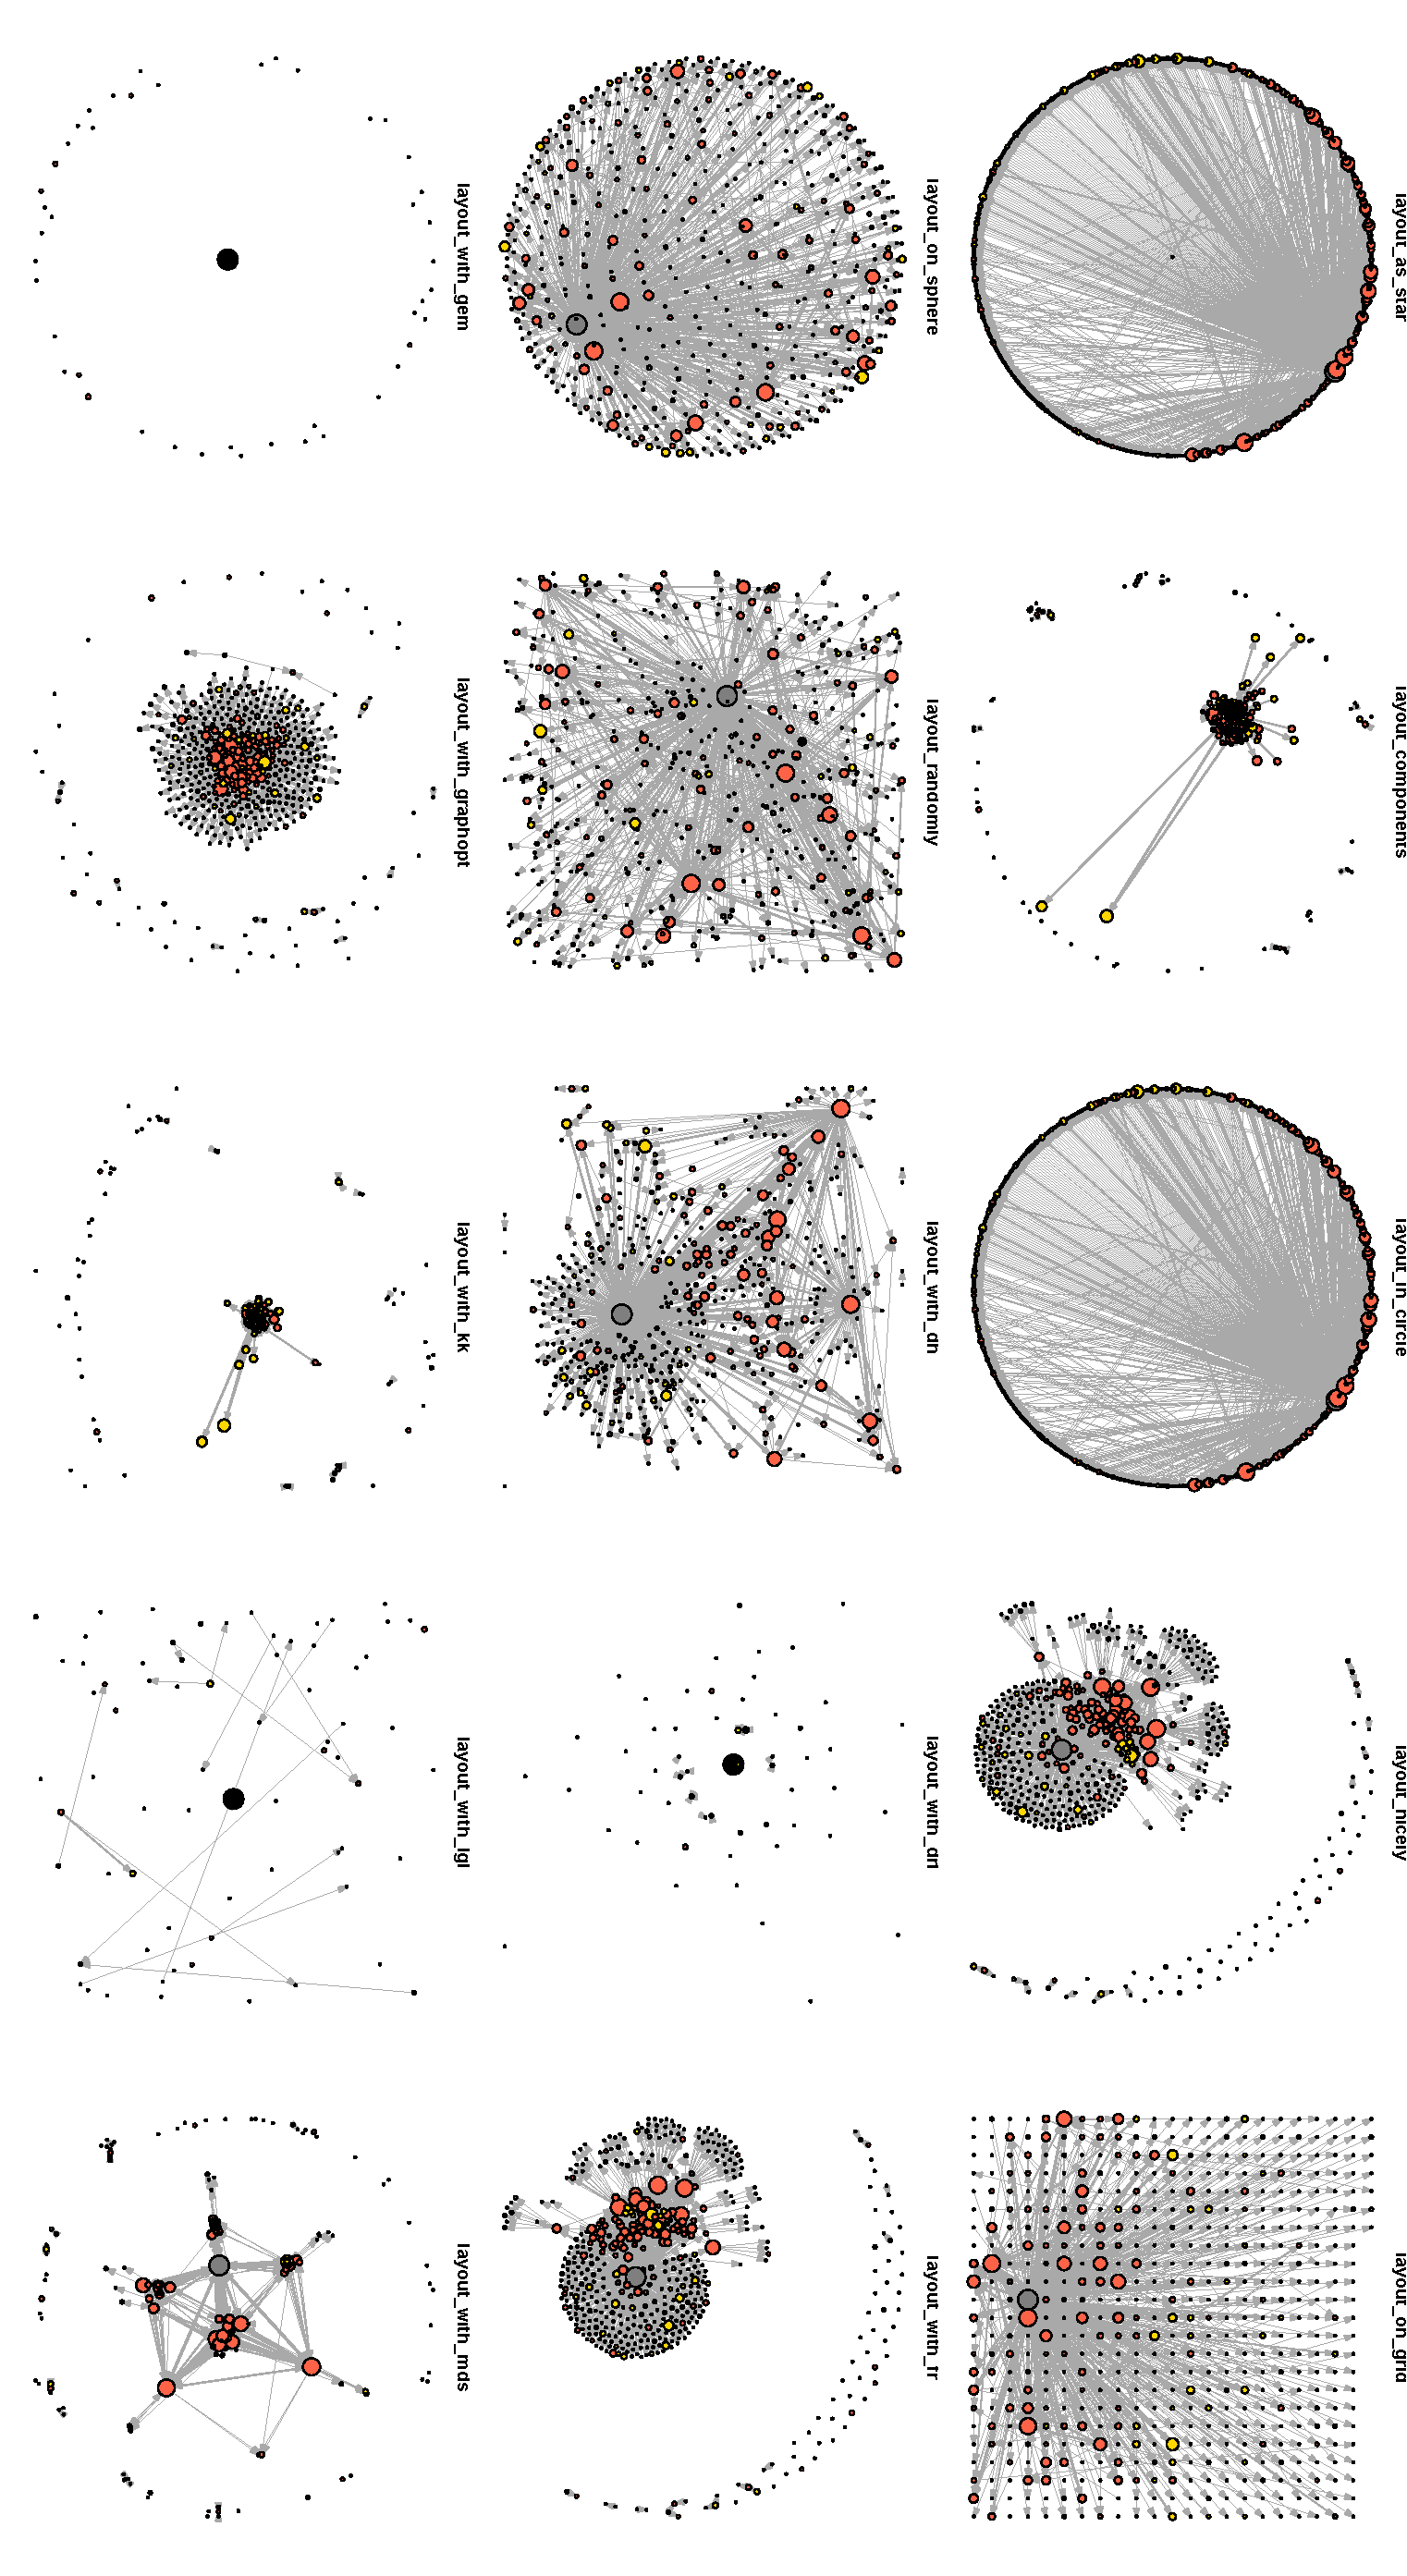
\includegraphics[width=.5\textwidth]{report_explore_layout}
\end{figure}
\subsection{Triads Summary}

\begin{table}
\centering
\begin{tabular}{l r} \hline
\bf Triad Type & \bf Frequency \\ \hline \hline
\verb+A,B,C+, the empty graph& 22105061 \\ 


\verb+A->B, C+, the graph with a single directed edge&173402 \\


\verb+A<->B, C+, the graph with a mutual connection between two vertices& 32376\\


\verb+A<-B->C+, the out-star &26006 \\


\verb+A->B<-C+, the in-star&1311 \\


\verb+A->B->C+, directed line&11609 \\


\verb+A<->B<-C+ &3205 \\


\verb+A<->B->C+&14505\\ 


\verb+A->B<-C, A->C+& 10 \\


\verb+A<-B<-C, A->C+ &0\\ 


\verb+A<->B<->C+ &1770 \\


\verb+A<-B->C, A<->C+ & 15\\


\verb+A->B<-C, A<->C+ & 65\\

\verb+A->B->C, A<->C+&24 \\

\verb+A->B<->C, A<->C+ &95\\


\verb+A<->B<->C, A<->C+ the complete graph&82

\end{tabular}
\end{table}


\subsection{Within Group Variation}
\begin{figure}[h!]
    \centering
    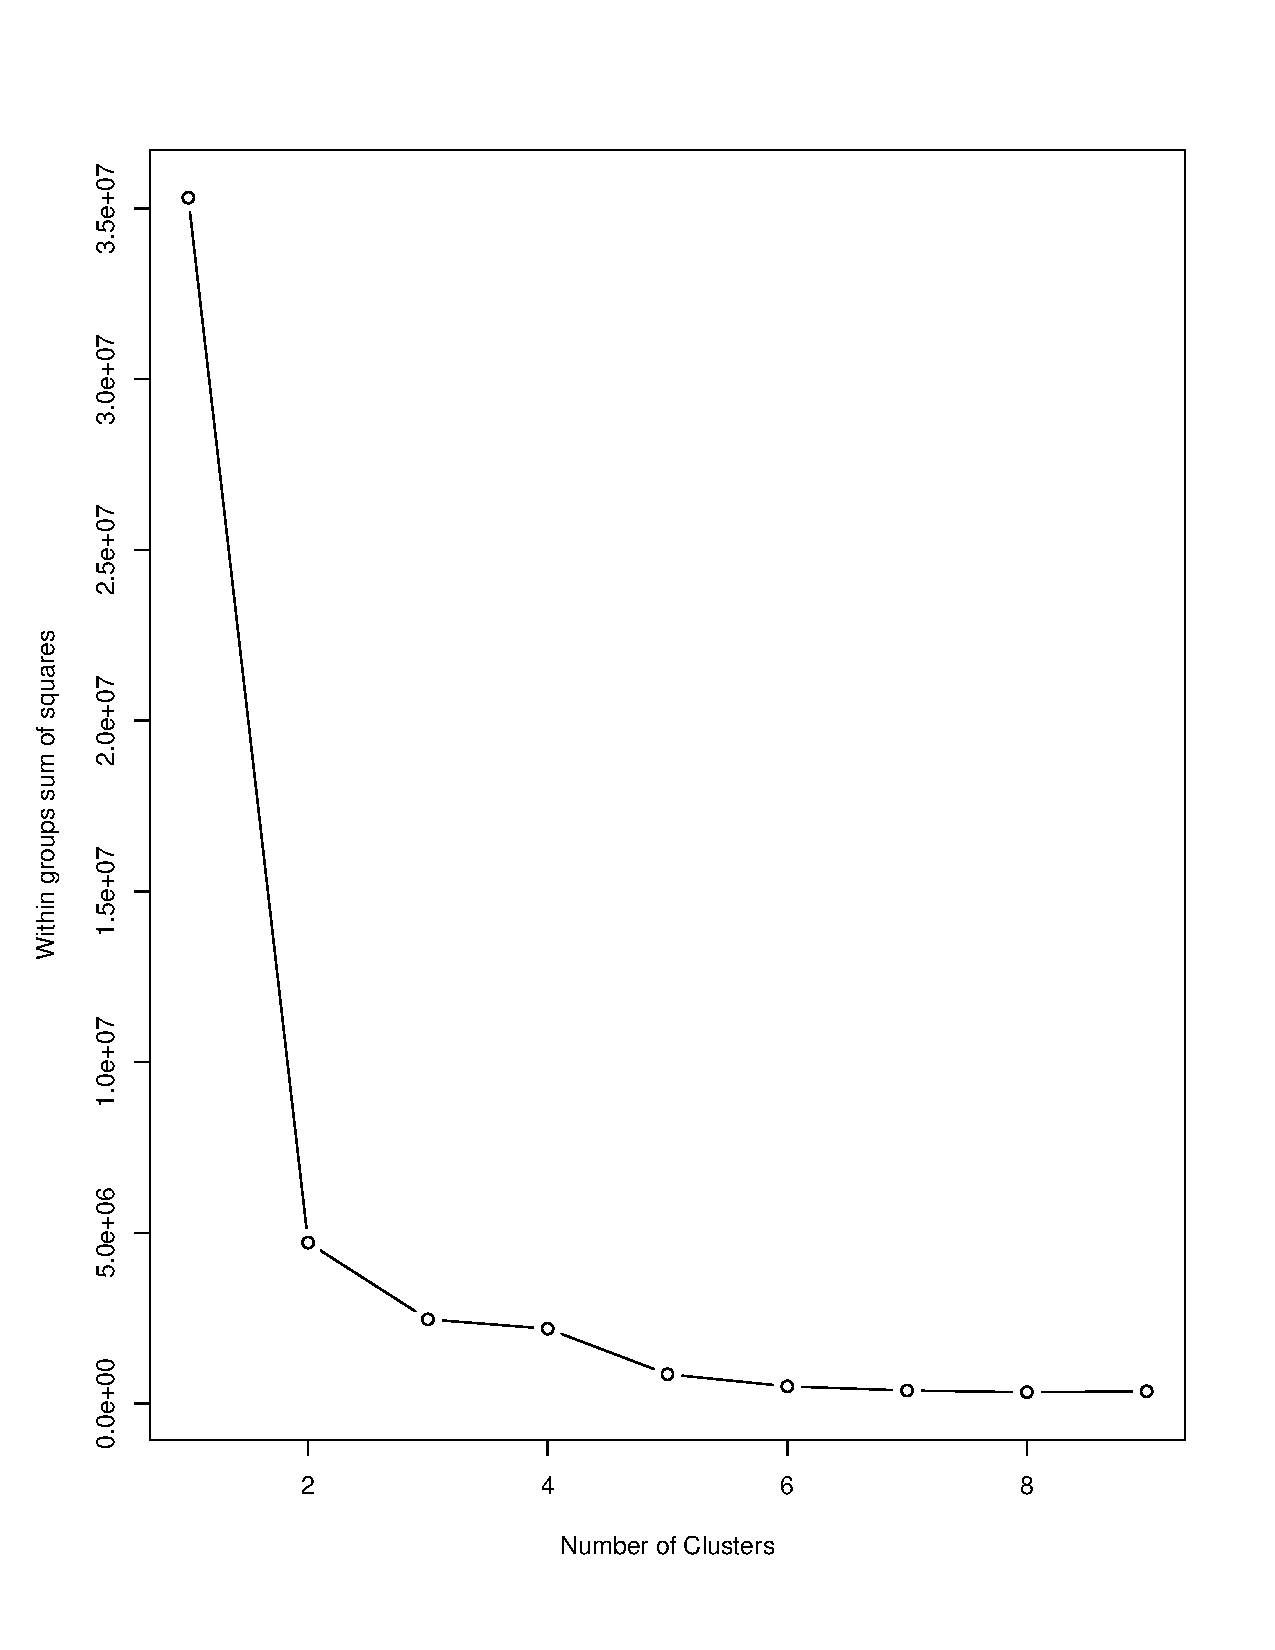
\includegraphics[width=10cm,height=10cm]
    {daitong_and_yihe/clusterd}
    \caption{Within Group Variation versus K=1,...,9}
    \label{fig:determine}
\end{figure}


\end{document}
